%&preformat-disser
\RequirePackage[l2tabu,orthodox]{nag} % Раскомментировав, можно в логе получать рекомендации относительно правильного использования пакетов и предупреждения об устаревших и нерекомендуемых пакетах
% Формат А4, 14pt (ГОСТ Р 7.0.11-2011, 5.3.6)
\documentclass[a4paper,14pt,oneside,openany]{memoir}

%%%%%%%%%%%%%%%%%%%%%%%%%%%%%%%%%%%%%%%%%%%%%%%%%%%%%%
%%%% Файл упрощённых настроек шаблона диссертации %%%%
%%%%%%%%%%%%%%%%%%%%%%%%%%%%%%%%%%%%%%%%%%%%%%%%%%%%%%

%%% Инициализирование переменных, не трогать!  %%%
\newcounter{intvl}
\newcounter{otstup}
\newcounter{contnumeq}
\newcounter{contnumfig}
\newcounter{contnumtab}
\newcounter{pgnum}
\newcounter{chapstyle}
\newcounter{headingdelim}
\newcounter{headingalign}
\newcounter{headingsize}
%%%%%%%%%%%%%%%%%%%%%%%%%%%%%%%%%%%%%%%%%%%%%%%%%%%%%%

%%% Область упрощённого управления оформлением %%%

%% Интервал между заголовками и между заголовком и текстом %%
% Заголовки отделяют от текста сверху и снизу
% тремя интервалами (ГОСТ Р 7.0.11-2011, 5.3.5)
\setcounter{intvl}{3}               % Коэффициент кратности к размеру шрифта

%% Отступы у заголовков в тексте %%
\setcounter{otstup}{0}              % 0 --- без отступа; 1 --- абзацный отступ

%% Нумерация формул, таблиц и рисунков %%
% Нумерация формул
\setcounter{contnumeq}{0}   % 0 --- пораздельно (во введении подряд,
                            %       без номера раздела);
                            % 1 --- сквозная нумерация по всей диссертации
% Нумерация рисунков
\setcounter{contnumfig}{0}  % 0 --- пораздельно (во введении подряд,
                            %       без номера раздела);
                            % 1 --- сквозная нумерация по всей диссертации
% Нумерация таблиц
\setcounter{contnumtab}{1}  % 0 --- пораздельно (во введении подряд,
                            %       без номера раздела);
                            % 1 --- сквозная нумерация по всей диссертации

%% Оглавление %%
\setcounter{pgnum}{1}       % 0 --- номера страниц никак не обозначены;
                            % 1 --- Стр. над номерами страниц (дважды
                            %       компилировать после изменения настройки)
\settocdepth{subsection}    % до какого уровня подразделов выносить в оглавление
\setsecnumdepth{subsection} % до какого уровня нумеровать подразделы


%% Текст и форматирование заголовков %%
\setcounter{chapstyle}{1}     % 0 --- разделы только под номером;
                              % 1 --- разделы с названием "Глава" перед номером
\setcounter{headingdelim}{1}  % 0 --- номер отделен пропуском в 1em или \quad;
                              % 1 --- номера разделов и приложений отделены
                              %       точкой с пробелом, подразделы пропуском
                              %       без точки;
                              % 2 --- номера разделов, подразделов и приложений
                              %       отделены точкой с пробелом.

%% Выравнивание заголовков в тексте %%
\setcounter{headingalign}{0}  % 0 --- по центру;
                              % 1 --- по левому краю

%% Размеры заголовков в тексте %%
\setcounter{headingsize}{0}   % 0 --- по ГОСТ, все всегда 14 пт;
                              % 1 --- пропорционально изменяющийся размер
                              %       в зависимости от базового шрифта

%% Подпись таблиц %%

% Смещение строк подписи после первой строки
\newcommand{\tabindent}{0cm}

% Тип форматирования заголовка таблицы:
% plain --- название и текст в одной строке
% split --- название и текст в разных строках
\newcommand{\tabformat}{plain}

%%% Настройки форматирования таблицы `plain`

% Выравнивание по центру подписи, состоящей из одной строки:
% true  --- выравнивать
% false --- не выравнивать
\newcommand{\tabsinglecenter}{false}

% Выравнивание подписи таблиц:
% justified   --- выравнивать как обычный текст («по ширине»)
% centering   --- выравнивать по центру
% centerlast  --- выравнивать по центру только последнюю строку
% centerfirst --- выравнивать по центру только первую строку (не рекомендуется)
% raggedleft  --- выравнивать по правому краю
% raggedright --- выравнивать по левому краю
\newcommand{\tabjust}{justified}

% Разделитель записи «Таблица #» и названия таблицы
\newcommand{\tablabelsep}{~\cyrdash\ }

%%% Настройки форматирования таблицы `split`

% Положение названия таблицы:
% \centering   --- выравнивать по центру
% \raggedleft  --- выравнивать по правому краю
% \raggedright --- выравнивать по левому краю
\newcommand{\splitformatlabel}{\raggedleft}

% Положение текста подписи:
% \centering   --- выравнивать по центру
% \raggedleft  --- выравнивать по правому краю
% \raggedright --- выравнивать по левому краю
\newcommand{\splitformattext}{\raggedright}

%% Подпись рисунков %%
%Разделитель записи «Рисунок #» и названия рисунка
\newcommand{\figlabelsep}{~\cyrdash\ }  % (ГОСТ 2.105, 4.3.1)
                                        % "--- здесь не работает

%%% Цвета гиперссылок %%%
% Latex color definitions: http://latexcolor.com/
%\definecolor{linkcolor}{rgb}{0.9,0,0}
%\definecolor{citecolor}{rgb}{0,0.6,0}
%\definecolor{urlcolor}{rgb}{0,0,1}
\definecolor{linkcolor}{rgb}{0,0,0} %black
\definecolor{citecolor}{rgb}{0,0,0} %black
\definecolor{urlcolor}{rgb}{0,0,0} %black
            % общие настройки шаблона
\input{common/packages}         % Пакеты общие для диссертации и автореферата
\synopsisfalse                      % Этот документ --- не автореферат
\input{Dissertation/dispackages}    % Пакеты для диссертации
\input{Dissertation/userpackages}   % Пакеты для специфических пользовательских задач

%%%%%%%%%%%%%%%%%%%%%%%%%%%%%%%%%%%%%%%%%%%%%%%%%%%%%%
%%%% Файл упрощённых настроек шаблона диссертации %%%%
%%%%%%%%%%%%%%%%%%%%%%%%%%%%%%%%%%%%%%%%%%%%%%%%%%%%%%

%%% Инициализирование переменных, не трогать!  %%%
\newcounter{intvl}
\newcounter{otstup}
\newcounter{contnumeq}
\newcounter{contnumfig}
\newcounter{contnumtab}
\newcounter{pgnum}
\newcounter{chapstyle}
\newcounter{headingdelim}
\newcounter{headingalign}
\newcounter{headingsize}
%%%%%%%%%%%%%%%%%%%%%%%%%%%%%%%%%%%%%%%%%%%%%%%%%%%%%%

%%% Область упрощённого управления оформлением %%%

%% Интервал между заголовками и между заголовком и текстом %%
% Заголовки отделяют от текста сверху и снизу
% тремя интервалами (ГОСТ Р 7.0.11-2011, 5.3.5)
\setcounter{intvl}{3}               % Коэффициент кратности к размеру шрифта

%% Отступы у заголовков в тексте %%
\setcounter{otstup}{0}              % 0 --- без отступа; 1 --- абзацный отступ

%% Нумерация формул, таблиц и рисунков %%
% Нумерация формул
\setcounter{contnumeq}{0}   % 0 --- пораздельно (во введении подряд,
                            %       без номера раздела);
                            % 1 --- сквозная нумерация по всей диссертации
% Нумерация рисунков
\setcounter{contnumfig}{0}  % 0 --- пораздельно (во введении подряд,
                            %       без номера раздела);
                            % 1 --- сквозная нумерация по всей диссертации
% Нумерация таблиц
\setcounter{contnumtab}{1}  % 0 --- пораздельно (во введении подряд,
                            %       без номера раздела);
                            % 1 --- сквозная нумерация по всей диссертации

%% Оглавление %%
\setcounter{pgnum}{1}       % 0 --- номера страниц никак не обозначены;
                            % 1 --- Стр. над номерами страниц (дважды
                            %       компилировать после изменения настройки)
\settocdepth{subsection}    % до какого уровня подразделов выносить в оглавление
\setsecnumdepth{subsection} % до какого уровня нумеровать подразделы


%% Текст и форматирование заголовков %%
\setcounter{chapstyle}{1}     % 0 --- разделы только под номером;
                              % 1 --- разделы с названием "Глава" перед номером
\setcounter{headingdelim}{1}  % 0 --- номер отделен пропуском в 1em или \quad;
                              % 1 --- номера разделов и приложений отделены
                              %       точкой с пробелом, подразделы пропуском
                              %       без точки;
                              % 2 --- номера разделов, подразделов и приложений
                              %       отделены точкой с пробелом.

%% Выравнивание заголовков в тексте %%
\setcounter{headingalign}{0}  % 0 --- по центру;
                              % 1 --- по левому краю

%% Размеры заголовков в тексте %%
\setcounter{headingsize}{0}   % 0 --- по ГОСТ, все всегда 14 пт;
                              % 1 --- пропорционально изменяющийся размер
                              %       в зависимости от базового шрифта

%% Подпись таблиц %%

% Смещение строк подписи после первой строки
\newcommand{\tabindent}{0cm}

% Тип форматирования заголовка таблицы:
% plain --- название и текст в одной строке
% split --- название и текст в разных строках
\newcommand{\tabformat}{plain}

%%% Настройки форматирования таблицы `plain`

% Выравнивание по центру подписи, состоящей из одной строки:
% true  --- выравнивать
% false --- не выравнивать
\newcommand{\tabsinglecenter}{false}

% Выравнивание подписи таблиц:
% justified   --- выравнивать как обычный текст («по ширине»)
% centering   --- выравнивать по центру
% centerlast  --- выравнивать по центру только последнюю строку
% centerfirst --- выравнивать по центру только первую строку (не рекомендуется)
% raggedleft  --- выравнивать по правому краю
% raggedright --- выравнивать по левому краю
\newcommand{\tabjust}{justified}

% Разделитель записи «Таблица #» и названия таблицы
\newcommand{\tablabelsep}{~\cyrdash\ }

%%% Настройки форматирования таблицы `split`

% Положение названия таблицы:
% \centering   --- выравнивать по центру
% \raggedleft  --- выравнивать по правому краю
% \raggedright --- выравнивать по левому краю
\newcommand{\splitformatlabel}{\raggedleft}

% Положение текста подписи:
% \centering   --- выравнивать по центру
% \raggedleft  --- выравнивать по правому краю
% \raggedright --- выравнивать по левому краю
\newcommand{\splitformattext}{\raggedright}

%% Подпись рисунков %%
%Разделитель записи «Рисунок #» и названия рисунка
\newcommand{\figlabelsep}{~\cyrdash\ }  % (ГОСТ 2.105, 4.3.1)
                                        % "--- здесь не работает

%%% Цвета гиперссылок %%%
% Latex color definitions: http://latexcolor.com/
%\definecolor{linkcolor}{rgb}{0.9,0,0}
%\definecolor{citecolor}{rgb}{0,0.6,0}
%\definecolor{urlcolor}{rgb}{0,0,1}
\definecolor{linkcolor}{rgb}{0,0,0} %black
\definecolor{citecolor}{rgb}{0,0,0} %black
\definecolor{urlcolor}{rgb}{0,0,0} %black
      % Упрощённые настройки шаблона

\input{common/newnames}         % Новые переменные, для всего проекта

%%% Основные сведения %%%
\newcommand{\thesisAuthorLastName}{Антонов}
\newcommand{\thesisAuthorOtherNames}{Илья Денисович}
\newcommand{\thesisAuthorInitials}{И.\,Д.}
\newcommand{\thesisAuthor}             % Диссертация, ФИО автора
{%
    \texorpdfstring{% \texorpdfstring takes two arguments and uses the first for (La)TeX and the second for pdf
        \thesisAuthorLastName~\thesisAuthorOtherNames% так будет отображаться на титульном листе или в тексте, где будет использоваться переменная
    }{%
        \thesisAuthorLastName, \thesisAuthorOtherNames% эта запись для свойств pdf-файла. В таком виде, если pdf будет обработан программами для сбора библиографических сведений, будет правильно представлена фамилия.
    }
}
\newcommand{\thesisAuthorShort}        % Диссертация, ФИО автора инициалами
{\thesisAuthorInitials~\thesisAuthorLastName}
%\newcommand{\thesisUdk}                % Диссертация, УДК
%{\fixme{xxx.xxx}}
\newcommand{\thesisTitle}              % Диссертация, название
{Проблемы управления нелинейными волновыми процессами в механических системах и численные методы их решения}
\newcommand{\thesisSpecialtyNumber}    % Диссертация, специальность, номер
{01.02.04}
\newcommand{\thesisSpecialtyTitle}     % Диссертация, специальность, название (название взято с сайта ВАК для примера)
{Механика деформируемого теврдого тела}
%% \newcommand{\thesisSpecialtyTwoNumber} % Диссертация, вторая специальность, номер
%% {\fixme{XX.XX.XX}}
%% \newcommand{\thesisSpecialtyTwoTitle}  % Диссертация, вторая специальность, название
%% {\fixme{Теория и~методика физического воспитания, спортивной тренировки,
%% оздоровительной и~адаптивной физической культуры}}
\newcommand{\thesisDegree}             % Диссертация, ученая степень
{кандидата физико-математических наук}
\newcommand{\thesisDegreeShort}        % Диссертация, ученая степень, краткая запись
{канд. физ.-мат. наук}
\newcommand{\thesisCity}               % Диссертация, город написания диссертации
{Санкт-Петербург}
\newcommand{\thesisYear}               % Диссертация, год написания диссертации
{\the\year}
\newcommand{\thesisOrganization}       % Диссертация, организация
{Федеральное государственное бюджетное учреждение науки <<Институт проблем машиноведения Российской академии наук <<ИПМаш РАН>>}
\newcommand{\thesisOrganizationShort}  % Диссертация, краткое название организации для доклада
{ИПМаш РАН}

\newcommand{\thesisInOrganization}     % Диссертация, организация в предложном падеже: Работа выполнена в ...
{институте проблем машиноведения Российской академии наук}

%% \newcommand{\supervisorDead}{}           % Рисовать рамку вокруг фамилии
\newcommand{\supervisorFio}              % Научный руководитель, ФИО
{Порубов Алексей Викторович}
\newcommand{\supervisorRegalia}          % Научный руководитель, регалии
{профессор, д-р~физ.-мат. наук}
\newcommand{\supervisorFioShort}         % Научный руководитель, ФИО
{А.\,В.~Порубов}
\newcommand{\supervisorRegaliaShort}     % Научный руководитель, регалии
{проф..,~д.ф.-м.н.}

%% \newcommand{\supervisorTwoDead}{}        % Рисовать рамку вокруг фамилии
%% \newcommand{\supervisorTwoFio}           % Второй научный руководитель, ФИО
%% {\fixme{Фамилия Имя Отчество}}
%% \newcommand{\supervisorTwoRegalia}       % Второй научный руководитель, регалии
%% {\fixme{уч. степень, уч. звание}}
%% \newcommand{\supervisorTwoFioShort}      % Второй научный руководитель, ФИО
%% {\fixme{И.\,О.~Фамилия}}
%% \newcommand{\supervisorTwoRegaliaShort}  % Второй научный руководитель, регалии
%% {\fixme{уч.~ст.,~уч.~зв.}}

\newcommand{\opponentOneFio}           % Оппонент 1, ФИО
{\fixme{Фамилия Имя Отчество}}
\newcommand{\opponentOneRegalia}       % Оппонент 1, регалии
{\fixme{доктор физико-математических наук, профессор}}
\newcommand{\opponentOneJobPlace}      % Оппонент 1, место работы
{\fixme{Не очень длинное название для места работы}}
\newcommand{\opponentOneJobPost}       % Оппонент 1, должность
{\fixme{старший научный сотрудник}}

\newcommand{\opponentTwoFio}           % Оппонент 2, ФИО
{\fixme{Фамилия Имя Отчество}}
\newcommand{\opponentTwoRegalia}       % Оппонент 2, регалии
{\fixme{кандидат физико-математических наук}}
\newcommand{\opponentTwoJobPlace}      % Оппонент 2, место работы
{\fixme{Основное место работы c длинным длинным длинным длинным названием}}
\newcommand{\opponentTwoJobPost}       % Оппонент 2, должность
{\fixme{старший научный сотрудник}}

%% \newcommand{\opponentThreeFio}         % Оппонент 3, ФИО
%% {\fixme{Фамилия Имя Отчество}}
%% \newcommand{\opponentThreeRegalia}     % Оппонент 3, регалии
%% {\fixme{кандидат физико-математических наук}}
%% \newcommand{\opponentThreeJobPlace}    % Оппонент 3, место работы
%% {\fixme{Основное место работы c длинным длинным длинным длинным названием}}
%% \newcommand{\opponentThreeJobPost}     % Оппонент 3, должность
%% {\fixme{старший научный сотрудник}}

%% \newcommand{\leadingOrganizationTitle} % Ведущая организация, дополнительные строки. Удалить, чтобы не отображать в автореферате
%% {\fixme{Федеральное государственное бюджетное образовательное учреждение высшего
%% профессионального образования с~длинным длинным длинным длинным названием}}

\newcommand{\defenseDate}              % Защита, дата
{\fixme{DD mmmmmmmm YYYY~г.~в~XX часов}}
\newcommand{\defenseCouncilNumber}     % Защита, номер диссертационного совета
{Д\,002.075.01}
\newcommand{\defenseCouncilTitle}      % Защита, учреждение диссертационного совета
{Институт проблем машиноведения Российской академии наук}
\newcommand{\defenseCouncilAddress}    % Защита, адрес учреждение диссертационного совета
{199178, г.Санкт-Петербург, Большой проспект В.О., д.61}
\newcommand{\defenseCouncilPhone}      % Телефон для справок
{+7~(812)~321-47-71}

\newcommand{\defenseSecretaryFio}      % Секретарь диссертационного совета, ФИО
{\fixme{Фамилия Имя Отчество}}
\newcommand{\defenseSecretaryRegalia}  % Секретарь диссертационного совета, регалии
{\fixme{д-р~физ.-мат. наук}}            % Для сокращений есть ГОСТы, например: ГОСТ Р 7.0.12-2011 + http://base.garant.ru/179724/#block_30000

\newcommand{\synopsisLibrary}          % Автореферат, название библиотеки
{\fixme{Название библиотеки}}
\newcommand{\synopsisDate}             % Автореферат, дата рассылки
{\fixme{DD mmmmmmmm}\the\year~года}

% To avoid conflict with beamer class use \providecommand
\providecommand{\keywords}%            % Ключевые слова для метаданных PDF диссертации и автореферата
{}
             % Основные сведения
\input{common/fonts}            % Определение шрифтов (частичное)
%%% Шаблон %%%
\DeclareRobustCommand{\fixme}{\textcolor{black}}  % решаем проблему превращения
                                % названия цвета в результате \MakeUppercase,
                                % http://tex.stackexchange.com/a/187930,
                                % \DeclareRobustCommand protects \fixme
                                % from expanding inside \MakeUppercase
\AtBeginDocument{%
    \setlength{\parindent}{2.5em}                   % Абзацный отступ. Должен быть одинаковым по всему тексту и равен пяти знакам (ГОСТ Р 7.0.11-2011, 5.3.7).
}

%%% Таблицы %%%
\DeclareCaptionLabelSeparator{tabsep}{\tablabelsep} % нумерация таблиц
\DeclareCaptionFormat{split}{\splitformatlabel#1\par\splitformattext#3}

\captionsetup[table]{
        format=\tabformat,                % формат подписи (plain|hang)
        font=normal,                      % нормальные размер, цвет, стиль шрифта
        skip=.0pt,                        % отбивка под подписью
        parskip=.0pt,                     % отбивка между параграфами подписи
        position=above,                   % положение подписи
        justification=\tabjust,           % центровка
        indent=\tabindent,                % смещение строк после первой
        labelsep=tabsep,                  % разделитель
        singlelinecheck=\tabsinglecenter, % не выравнивать по центру, если умещается в одну строку
}

%%% Рисунки %%%
\DeclareCaptionLabelSeparator{figsep}{\figlabelsep} % нумерация рисунков

\captionsetup[figure]{
        format=plain,                     % формат подписи (plain|hang)
        font=normal,                      % нормальные размер, цвет, стиль шрифта
        skip=.0pt,                        % отбивка под подписью
        parskip=.0pt,                     % отбивка между параграфами подписи
        position=below,                   % положение подписи
        singlelinecheck=true,             % выравнивание по центру, если умещается в одну строку
        justification=centerlast,         % центровка
        labelsep=figsep,                  % разделитель
}

%%% Подписи подрисунков %%%
\DeclareCaptionSubType{figure}
\renewcommand\thesubfigure{\asbuk{subfigure}} % нумерация подрисунков
\ifsynopsis
\DeclareCaptionFont{norm}{\fontsize{10pt}{11pt}\selectfont}
\newcommand{\subfigureskip}{2.pt}
\else
\DeclareCaptionFont{norm}{\fontsize{14pt}{16pt}\selectfont}
\newcommand{\subfigureskip}{0.pt}
\fi

\captionsetup[subfloat]{
        labelfont=norm,                 % нормальный размер подписей подрисунков
        textfont=norm,                  % нормальный размер подписей подрисунков
        labelsep=space,                 % разделитель
        labelformat=brace,              % одна скобка справа от номера
        justification=centering,        % центровка
        singlelinecheck=true,           % выравнивание по центру, если умещается в одну строку
        skip=\subfigureskip,            % отбивка над подписью
        parskip=.0pt,                   % отбивка между параграфами подписи
        position=below,                 % положение подписи
}

%%% Настройки ссылок на рисунки, таблицы и др. %%%
% команды \cref...format отвечают за форматирование при помощи команды \cref
% команды \labelcref...format отвечают за форматирование при помощи команды \labelcref

\ifpresentation
\else
    \crefdefaultlabelformat{#2#1#3}

    % Уравнение
    \crefformat{equation}{(#2#1#3)} % одиночная ссылка с приставкой
    \labelcrefformat{equation}{(#2#1#3)} % одиночная ссылка без приставки
    \crefrangeformat{equation}{(#3#1#4) \cyrdash~(#5#2#6)} % диапазон ссылок с приставкой
    \labelcrefrangeformat{equation}{(#3#1#4) \cyrdash~(#5#2#6)} % диапазон ссылок без приставки
    \crefmultiformat{equation}{(#2#1#3)}{ и~(#2#1#3)}{, (#2#1#3)}{ и~(#2#1#3)} % перечисление ссылок с приставкой
    \labelcrefmultiformat{equation}{(#2#1#3)}{ и~(#2#1#3)}{, (#2#1#3)}{ и~(#2#1#3)} % перечисление без приставки

    % Подуравнение
    \crefformat{subequation}{(#2#1#3)} % одиночная ссылка с приставкой
    \labelcrefformat{subequation}{(#2#1#3)} % одиночная ссылка без приставки
    \crefrangeformat{subequation}{(#3#1#4) \cyrdash~(#5#2#6)} % диапазон ссылок с приставкой
    \labelcrefrangeformat{subequation}{(#3#1#4) \cyrdash~(#5#2#6)} % диапазон ссылок без приставки
    \crefmultiformat{subequation}{(#2#1#3)}{ и~(#2#1#3)}{, (#2#1#3)}{ и~(#2#1#3)} % перечисление ссылок с приставкой
    \labelcrefmultiformat{subequation}{(#2#1#3)}{ и~(#2#1#3)}{, (#2#1#3)}{ и~(#2#1#3)} % перечисление без приставки

    % Глава
    \crefformat{chapter}{#2#1#3} % одиночная ссылка с приставкой
    \labelcrefformat{chapter}{#2#1#3} % одиночная ссылка без приставки
    \crefrangeformat{chapter}{#3#1#4 \cyrdash~#5#2#6} % диапазон ссылок с приставкой
    \labelcrefrangeformat{chapter}{#3#1#4 \cyrdash~#5#2#6} % диапазон ссылок без приставки
    \crefmultiformat{chapter}{#2#1#3}{ и~#2#1#3}{, #2#1#3}{ и~#2#1#3} % перечисление ссылок с приставкой
    \labelcrefmultiformat{chapter}{#2#1#3}{ и~#2#1#3}{, #2#1#3}{ и~#2#1#3} % перечисление без приставки

    % Параграф
    \crefformat{section}{#2#1#3} % одиночная ссылка с приставкой
    \labelcrefformat{section}{#2#1#3} % одиночная ссылка без приставки
    \crefrangeformat{section}{#3#1#4 \cyrdash~#5#2#6} % диапазон ссылок с приставкой
    \labelcrefrangeformat{section}{#3#1#4 \cyrdash~#5#2#6} % диапазон ссылок без приставки
    \crefmultiformat{section}{#2#1#3}{ и~#2#1#3}{, #2#1#3}{ и~#2#1#3} % перечисление ссылок с приставкой
    \labelcrefmultiformat{section}{#2#1#3}{ и~#2#1#3}{, #2#1#3}{ и~#2#1#3} % перечисление без приставки

    % Приложение
    \crefformat{appendix}{#2#1#3} % одиночная ссылка с приставкой
    \labelcrefformat{appendix}{#2#1#3} % одиночная ссылка без приставки
    \crefrangeformat{appendix}{#3#1#4 \cyrdash~#5#2#6} % диапазон ссылок с приставкой
    \labelcrefrangeformat{appendix}{#3#1#4 \cyrdash~#5#2#6} % диапазон ссылок без приставки
    \crefmultiformat{appendix}{#2#1#3}{ и~#2#1#3}{, #2#1#3}{ и~#2#1#3} % перечисление ссылок с приставкой
    \labelcrefmultiformat{appendix}{#2#1#3}{ и~#2#1#3}{, #2#1#3}{ и~#2#1#3} % перечисление без приставки

    % Рисунок
    \crefformat{figure}{#2#1#3} % одиночная ссылка с приставкой
    \labelcrefformat{figure}{#2#1#3} % одиночная ссылка без приставки
    \crefrangeformat{figure}{#3#1#4 \cyrdash~#5#2#6} % диапазон ссылок с приставкой
    \labelcrefrangeformat{figure}{#3#1#4 \cyrdash~#5#2#6} % диапазон ссылок без приставки
    \crefmultiformat{figure}{#2#1#3}{ и~#2#1#3}{, #2#1#3}{ и~#2#1#3} % перечисление ссылок с приставкой
    \labelcrefmultiformat{figure}{#2#1#3}{ и~#2#1#3}{, #2#1#3}{ и~#2#1#3} % перечисление без приставки

    % Таблица
    \crefformat{table}{#2#1#3} % одиночная ссылка с приставкой
    \labelcrefformat{table}{#2#1#3} % одиночная ссылка без приставки
    \crefrangeformat{table}{#3#1#4 \cyrdash~#5#2#6} % диапазон ссылок с приставкой
    \labelcrefrangeformat{table}{#3#1#4 \cyrdash~#5#2#6} % диапазон ссылок без приставки
    \crefmultiformat{table}{#2#1#3}{ и~#2#1#3}{, #2#1#3}{ и~#2#1#3} % перечисление ссылок с приставкой
    \labelcrefmultiformat{table}{#2#1#3}{ и~#2#1#3}{, #2#1#3}{ и~#2#1#3} % перечисление без приставки

    % Листинг
    \crefformat{lstlisting}{#2#1#3} % одиночная ссылка с приставкой
    \labelcrefformat{lstlisting}{#2#1#3} % одиночная ссылка без приставки
    \crefrangeformat{lstlisting}{#3#1#4 \cyrdash~#5#2#6} % диапазон ссылок с приставкой
    \labelcrefrangeformat{lstlisting}{#3#1#4 \cyrdash~#5#2#6} % диапазон ссылок без приставки
    \crefmultiformat{lstlisting}{#2#1#3}{ и~#2#1#3}{, #2#1#3}{ и~#2#1#3} % перечисление ссылок с приставкой
    \labelcrefmultiformat{lstlisting}{#2#1#3}{ и~#2#1#3}{, #2#1#3}{ и~#2#1#3} % перечисление без приставки

    % Листинг
    \crefformat{ListingEnv}{#2#1#3} % одиночная ссылка с приставкой
    \labelcrefformat{ListingEnv}{#2#1#3} % одиночная ссылка без приставки
    \crefrangeformat{ListingEnv}{#3#1#4 \cyrdash~#5#2#6} % диапазон ссылок с приставкой
    \labelcrefrangeformat{ListingEnv}{#3#1#4 \cyrdash~#5#2#6} % диапазон ссылок без приставки
    \crefmultiformat{ListingEnv}{#2#1#3}{ и~#2#1#3}{, #2#1#3}{ и~#2#1#3} % перечисление ссылок с приставкой
    \labelcrefmultiformat{ListingEnv}{#2#1#3}{ и~#2#1#3}{, #2#1#3}{ и~#2#1#3} % перечисление без приставки
\fi

%%% Настройки гиперссылок %%%
\ifluatex
    \hypersetup{
        unicode,                % Unicode encoded PDF strings
    }
\fi

\hypersetup{
    linktocpage=true,           % ссылки с номера страницы в оглавлении, списке таблиц и списке рисунков
%    linktoc=all,                % both the section and page part are links
%    pdfpagelabels=false,        % set PDF page labels (true|false)
    plainpages=false,           % Forces page anchors to be named by the Arabic form  of the page number, rather than the formatted form
    colorlinks,                 % ссылки отображаются раскрашенным текстом, а не раскрашенным прямоугольником, вокруг текста
    linkcolor={linkcolor},      % цвет ссылок типа ref, eqref и подобных
    citecolor={citecolor},      % цвет ссылок-цитат
    urlcolor={urlcolor},        % цвет гиперссылок
%    hidelinks,                  % Hide links (removing color and border)
    pdftitle={\thesisTitle},    % Заголовок
    pdfauthor={\thesisAuthor},  % Автор
    pdfsubject={\thesisSpecialtyNumber\ \thesisSpecialtyTitle},      % Тема
%    pdfcreator={Создатель},     % Создатель, Приложение
%    pdfproducer={Производитель},% Производитель, Производитель PDF
    pdfkeywords={\keywords},    % Ключевые слова
    pdflang={ru},
}
\ifnumequal{\value{draft}}{1}{% Черновик
    \hypersetup{
        draft,
    }
}{}

%%% Списки %%%
% Используем короткое тире (endash) для ненумерованных списков (ГОСТ 2.105-95, пункт 4.1.7, требует дефиса, но так лучше смотрится)
\renewcommand{\labelitemi}{\normalfont\bfseries{--}}

% Перечисление строчными буквами латинского алфавита (ГОСТ 2.105-95, 4.1.7)
%\renewcommand{\theenumi}{\alph{enumi}}
%\renewcommand{\labelenumi}{\theenumi)}

% Перечисление строчными буквами русского алфавита (ГОСТ 2.105-95, 4.1.7)
\makeatletter
\AddEnumerateCounter{\asbuk}{\russian@alph}{щ}      % Управляем списками/перечислениями через пакет enumitem, а он 'не знает' про asbuk, потому 'учим' его
\makeatother
%\renewcommand{\theenumi}{\asbuk{enumi}} %первый уровень нумерации
%\renewcommand{\labelenumi}{\theenumi)} %первый уровень нумерации
\renewcommand{\theenumii}{\asbuk{enumii}} %второй уровень нумерации
\renewcommand{\labelenumii}{\theenumii)} %второй уровень нумерации
\renewcommand{\theenumiii}{\arabic{enumiii}} %третий уровень нумерации
\renewcommand{\labelenumiii}{\theenumiii)} %третий уровень нумерации

\setlist{nosep,%                                    % Единый стиль для всех списков (пакет enumitem), без дополнительных интервалов.
    labelindent=\parindent,leftmargin=*%            % Каждый пункт, подпункт и перечисление записывают с абзацного отступа (ГОСТ 2.105-95, 4.1.8)
}

%%% Правильная нумерация приложений, рисунков и формул %%%
%% По ГОСТ 2.105, п. 4.3.8 Приложения обозначают заглавными буквами русского алфавита,
%% начиная с А, за исключением букв Ё, З, Й, О, Ч, Ь, Ы, Ъ.
%% Здесь также переделаны все нумерации русскими буквами.
\ifxetexorluatex
    \makeatletter
    \def\russian@Alph#1{\ifcase#1\or
       А\or Б\or В\or Г\or Д\or Е\or Ж\or
       И\or К\or Л\or М\or Н\or
       П\or Р\or С\or Т\or У\or Ф\or Х\or
       Ц\or Ш\or Щ\or Э\or Ю\or Я\else\xpg@ill@value{#1}{russian@Alph}\fi}
    \def\russian@alph#1{\ifcase#1\or
       а\or б\or в\or г\or д\or е\or ж\or
       и\or к\or л\or м\or н\or
       п\or р\or с\or т\or у\or ф\or х\or
       ц\or ш\or щ\or э\or ю\or я\else\xpg@ill@value{#1}{russian@alph}\fi}
    \def\cyr@Alph#1{\ifcase#1\or
        А\or Б\or В\or Г\or Д\or Е\or Ж\or
        И\or К\or Л\or М\or Н\or
        П\or Р\or С\or Т\or У\or Ф\or Х\or
        Ц\or Ш\or Щ\or Э\or Ю\or Я\else\xpg@ill@value{#1}{cyr@Alph}\fi}
    \def\cyr@alph#1{\ifcase#1\or
        а\or б\or в\or г\or д\or е\or ж\or
        и\or к\or л\or м\or н\or
        п\or р\or с\or т\or у\or ф\or х\or
        ц\or ш\or щ\or э\or ю\or я\else\xpg@ill@value{#1}{cyr@alph}\fi}
    \makeatother
\else
    \makeatletter
    \if@uni@ode
      \def\russian@Alph#1{\ifcase#1\or
        А\or Б\or В\or Г\or Д\or Е\or Ж\or
        И\or К\or Л\or М\or Н\or
        П\or Р\or С\or Т\or У\or Ф\or Х\or
        Ц\or Ш\or Щ\or Э\or Ю\or Я\else\@ctrerr\fi}
    \else
      \def\russian@Alph#1{\ifcase#1\or
        \CYRA\or\CYRB\or\CYRV\or\CYRG\or\CYRD\or\CYRE\or\CYRZH\or
        \CYRI\or\CYRK\or\CYRL\or\CYRM\or\CYRN\or
        \CYRP\or\CYRR\or\CYRS\or\CYRT\or\CYRU\or\CYRF\or\CYRH\or
        \CYRC\or\CYRSH\or\CYRSHCH\or\CYREREV\or\CYRYU\or
        \CYRYA\else\@ctrerr\fi}
    \fi
    \if@uni@ode
      \def\russian@alph#1{\ifcase#1\or
        а\or б\or в\or г\or д\or е\or ж\or
        и\or к\or л\or м\or н\or
        п\or р\or с\or т\or у\or ф\or х\or
        ц\or ш\or щ\or э\or ю\or я\else\@ctrerr\fi}
    \else
      \def\russian@alph#1{\ifcase#1\or
        \cyra\or\cyrb\or\cyrv\or\cyrg\or\cyrd\or\cyre\or\cyrzh\or
        \cyri\or\cyrk\or\cyrl\or\cyrm\or\cyrn\or
        \cyrp\or\cyrr\or\cyrs\or\cyrt\or\cyru\or\cyrf\or\cyrh\or
        \cyrc\or\cyrsh\or\cyrshch\or\cyrerev\or\cyryu\or
        \cyrya\else\@ctrerr\fi}
    \fi
    \makeatother
\fi


%%http://www.linux.org.ru/forum/general/6993203#comment-6994589 (используется totcount)
\makeatletter
\def\formtotal#1#2#3#4#5{%
    \newcount\@c
    \@c\totvalue{#1}\relax
    \newcount\@last
    \newcount\@pnul
    \@last\@c\relax
    \divide\@last 10
    \@pnul\@last\relax
    \divide\@pnul 10
    \multiply\@pnul-10
    \advance\@pnul\@last
    \multiply\@last-10
    \advance\@last\@c
    #2%
    \ifnum\@pnul=1#5\else%
    \ifcase\@last#5\or#3\or#4\or#4\or#4\else#5\fi
    \fi
}
\makeatother

\newcommand{\formbytotal}[5]{\total{#1}~\formtotal{#1}{#2}{#3}{#4}{#5}}

%%% Команды рецензирования %%%
\ifboolexpr{ (test {\ifnumequal{\value{draft}}{1}}) or (test {\ifnumequal{\value{showmarkup}}{1}})}{
        \newrobustcmd{\todo}[1]{\textcolor{red}{#1}}
        \newrobustcmd{\note}[2][]{\ifstrempty{#1}{#2}{\textcolor{#1}{#2}}}
        \newenvironment{commentbox}[1][]%
        {\ifstrempty{#1}{}{\color{#1}}}%
        {}
}{
        \newrobustcmd{\todo}[1]{}
        \newrobustcmd{\note}[2][]{}
        \excludecomment{commentbox}
}
           % Стили общие для диссертации и автореферата
\input{Dissertation/disstyles}  % Стили для диссертации
\input{Dissertation/userstyles} % Стили для специфических пользовательских задач

%%% Библиография. Выбор движка для реализации %%%
% Здесь только проверка установленного ключа. Сама настройка выбора движка
% размещена в common/setup.tex
\ifnumequal{\value{bibliosel}}{0}{%
    \input{biblio/predefined}   % Встроенная реализация с загрузкой файла через движок bibtex8
}{
    \input{biblio/biblatex}     % Реализация пакетом biblatex через движок biber
}

% Вывести информацию о выбранных опциях в лог сборки
\typeout{Selected options:}
\typeout{Draft mode: \arabic{draft}}
\typeout{Font: \arabic{fontfamily}}
\typeout{AltFont: \arabic{usealtfont}}
\typeout{Bibliography backend: \arabic{bibliosel}}
\typeout{Precompile images: \arabic{imgprecompile}}
% Вывести информацию о версиях используемых библиотек в лог сборки
\listfiles

%%% Управление компиляцией отдельных частей диссертации %%%
% Необходимо сначала иметь полностью скомпилированный документ, чтобы все
% промежуточные файлы были в наличии
% Затем, для вывода отдельных частей можно воспользоваться командой \includeonly
% Ниже примеры использования команды:
%
%\includeonly{Dissertation/part2}
%\includeonly{Dissertation/contents,Dissertation/appendix,Dissertation/conclusion}
%
% Если все команды закомментированы, то документ будет выведен в PDF файл полностью

\begin{document}
%%% Переопределение именований типовых разделов
% https://tex.stackexchange.com/a/156050
\gappto\captionsrussian{\input{common/renames}\unskip} % for polyglossia and babel
\input{common/renames}

%%% Структура диссертации (ГОСТ Р 7.0.11-2011, 4)
% Титульный лист (ГОСТ Р 7.0.11-2001, 5.1)
\thispagestyle{empty}
\begin{center}
\thesisOrganization
\end{center}
%
\vspace{0pt plus4fill} %число перед fill = кратность относительно некоторого расстояния fill, кусками которого заполнены пустые места
\IfFileExists{images/logo.pdf}{
  \begin{minipage}[b]{0.5\linewidth}
    \begin{flushleft}
%%      \includegraphics[height=3.5cm]{logo}
    \end{flushleft}
  \end{minipage}%
  \begin{minipage}[b]{0.5\linewidth}
    \begin{flushright}
      На правах рукописи\\
%      \textsl {УДК \thesisUdk}
    \end{flushright}
  \end{minipage}
}{
\begin{flushright}
На правах рукописи

%\textsl {УДК \thesisUdk}
\end{flushright}
}
%
\vspace{0pt plus6fill} %число перед fill = кратность относительно некоторого расстояния fill, кусками которого заполнены пустые места
\begin{center}
{\large \thesisAuthor}
\end{center}
%
\vspace{0pt plus1fill} %число перед fill = кратность относительно некоторого расстояния fill, кусками которого заполнены пустые места
\begin{center}
\textbf {\large %\MakeUppercase
\thesisTitle}

\vspace{0pt plus2fill} %число перед fill = кратность относительно некоторого расстояния fill, кусками которого заполнены пустые места
{%\small
Специальность \thesisSpecialtyNumber\ "---

<<\thesisSpecialtyTitle>>
}

\ifdefined\thesisSpecialtyTwoNumber
{%\small
Специальность \thesisSpecialtyTwoNumber\ "---

<<\thesisSpecialtyTwoTitle>>
}
\fi

\vspace{0pt plus2fill} %число перед fill = кратность относительно некоторого расстояния fill, кусками которого заполнены пустые места
Диссертация на соискание учёной степени

\thesisDegree
\end{center}
%
\vspace{0pt plus4fill} %число перед fill = кратность относительно некоторого расстояния fill, кусками которого заполнены пустые места
\begin{flushright}
\ifdefined\supervisorTwoFio
Научные руководители:

\supervisorRegalia

\ifdefined\supervisorDead
\framebox{\supervisorFio}
\else
\supervisorFio
\fi

\supervisorTwoRegalia

\ifdefined\supervisorTwoDead
\framebox{\supervisorTwoFio}
\else
\supervisorTwoFio
\fi
\else
Научный руководитель:

\supervisorRegalia

\ifdefined\supervisorDead
\framebox{\supervisorFio}
\else
\supervisorFio
\fi
\fi

\end{flushright}
%
\vspace{0pt plus4fill} %число перед fill = кратность относительно некоторого расстояния fill, кусками которого заполнены пустые места
{\centering\thesisCity\ "--- \thesisYear\par}
           % Титульный лист
\include{Dissertation/contents}        % Оглавление
\ifnumequal{\value{contnumfig}}{1}{}{\counterwithout{figure}{chapter}}
\ifnumequal{\value{contnumtab}}{1}{}{\counterwithout{table}{chapter}}
\chapter*{Введение}                         % Заголовок
\addcontentsline{toc}{chapter}{Введение}    % Добавляем его в оглавление

\newcommand{\actuality}{}
\newcommand{\progress}{}
\newcommand{\aim}{{\textbf\aimTXT}}
\newcommand{\tasks}{\textbf{\tasksTXT}}
\newcommand{\novelty}{\textbf{\noveltyTXT}}
\newcommand{\influence}{\textbf{\influenceTXT}}
\newcommand{\methods}{\textbf{\methodsTXT}}
\newcommand{\defpositions}{\textbf{\defpositionsTXT}}
\newcommand{\reliability}{\textbf{\reliabilityTXT}}
\newcommand{\probation}{\textbf{\probationTXT}}
\newcommand{\contribution}{\textbf{\contributionTXT}}
\newcommand{\publications}{\textbf{\publicationsTXT}}


%{\actuality} Обзор, введение в тему, обозначение места данной работы в мировых исследованиях и~т.\:п., можно использовать ссылки на~другие работы~\autocite{Gosele1999161,Lermontov} (если их~нет, то~в~автореферате автоматически пропадёт раздел <<Список литературы>>). Внимание! Ссылки на~другие работы в~разделе общей характеристики работы можно использовать только при использовании \verb!biblatex! (из-за технических ограничений \verb!bibtex8!. Это связано с тем, что одна и~та~же~характеристика используются и~в~тексте диссертации, и в автореферате. В~последнем, согласно ГОСТ, должен присутствовать список работ автора по~теме диссертации, а~\verb!bibtex8! не~умеет выводить в~одном файле два списка литературы). При использовании \verb!biblatex! возможно использование исключительно в~автореферате подстрочных ссылок для других работ командой \verb!\autocite!, а~также цитирование собственных работ командой \verb!\cite!. Для этого в~файле \verb!common/setup.tex! необходимо присвоить положительное значение счётчику \verb!\setcounter{usefootcite}{1}!.

Работа посвящена исследованию волновых процессов в сложных механических структурах и управлению ими. К таковым, с одной стороны отнесены нелинейные динамические процессы в материалах со сложной структурой: в <<двухатомном>> слое ограниченной толщины и двумерной обобщенной решетке, уравнения движения которых выведены с использованием вариационного принципа Гамильтона-Остроградского и ряда асимптотических процедур. В случае двумерного слоя особое внимание уделяется свойствам модельных уравнений движения и численным методам их исследования, вопросам существования и распространения локализованных волн деформации в рассматриваемых материалах, а также возможности локализации таких волн или изменения их параметров средствами управляющих воздействий, оказываемых влиянием внешней нагрузки, обратная связь для которых обеспечивается выбором граничных условий. Вид функции потенциальной энергии определяется ранее разработанной нелинейной моделью \cite{bound_porsp17}, выведенной на основе рассмотрения механической задачи о дискретной двухатомной решетке. Вид управляющей функции с обратной связью был предложен и апробирован в серии предшествующих работ \cite{porant16,porant17,PorubovAntonov2018mechSystem} и определяется согласно методу скоростного градиента \cite{fradkov_rus_speed_grad}. В случае решетки, за основу берется ранее разработанная модель \cite{porkros}, численно исследуются вопросы поперечной устойчивости локализованных решений уравнения движения для сдвиговых волн, которое является обобщением уравнения Кадомцева-Петвиашвили \cite{kadpet} с дополнительным интегральным слагаемым. Для учета последнего в работе предлагается спектральный численный метод, исследуются границы его применимости.

С другой стороны, к таковым отнесены линейные акустические (механические) метаматериалы, рассматривается известная модель цепочки <<масса в массе>> \cite{Huang2009}. Численно исследуются вопросы генерации гармонических волн, влияние запрещенной зоны на их распространение, возможность влияния на волны внешним воздействием, а \fixme{также обсуждается обобщение модели на учет нелинейных эффектов и соответствующих численных моделей}. Полученные результаты могут быть воспроизведены на экспериментальных установках и использоваться для дальнейших теоретических и практических исследований в области наук о метаматериалах.

{\actuality} Наука о нелинейных волновых процессах в механических системах имеют богатую историю. При этом в последнее время растет интерес к возможности управления этими процессами все в более сложных системах, которое открывает новые перспективы развития в бурно развивающейся области методов акустического неразрушающего контроля с целью измерения прочностных свойств, выявления дефектов и других параметров материалов. Активные исследования акустических метаматериалов, и модели <<масса-в-массе>> в частности, зародились и бурно развивались в рамках последнего десятилетия, открывая возможности для обнаружения и разработки новых материалов с уникальными свойствами. Перечисленные факты более чем подтверждают \textbf{актуальность} исследований, проводимых в данной работе.

%Для генерации содержимого титульного листа автореферата, диссертации и~презентации используются данные из файла \verb!common/data.tex!. Если, например, вы меняете название диссертации, то оно автоматически появится в~итоговых файлах после очередного запуска \LaTeX. Согласно ГОСТ 7.0.11-2011 <<5.1.1 Титульный лист является первой страницей диссертации, служит источником информации, необходимой для обработки и поиска документа>>. Наличие логотипа организации на~титульном листе упрощает обработку и~поиск, для этого разметите логотип вашей организации в папке images в~формате PDF (лучше найти его в векторном варианте, чтобы он хорошо смотрелся при печати) под именем \verb!logo.pdf!. Настроить размер изображения с логотипом можно в~соответствующих местах файлов \verb!title.tex!  отдельно для диссертации и автореферата. Если вам логотип не~нужен, то просто удалите файл с~логотипом.

%\ifsynopsis
%Этот абзац появляется только в~автореферате.
%Для формирования блоков, которые будут обрабатываться только в~автореферате,
%заведена проверка условия \verb!\!\verb!ifsynopsis!.
%Значение условия задаётся в~основном файле документа (\verb!synopsis.tex! для
%автореферата).
%\else
%Этот абзац появляется только в~диссертации.
%Через проверку условия \verb!\!\verb!ifsynopsis!, задаваемого в~основном файле
%документа (\verb!dissertation.tex! для диссертации), можно сделать новую
%команду, обеспечивающую появление цитаты в~диссертации, но~не~в~автореферате.
%\fi

% {\progress}
% Этот раздел должен быть отдельным структурным элементом по
% ГОСТ, но он, как правило, включается в описание актуальности
% темы. Нужен он отдельным структурынм элемементом или нет ---
% смотрите другие диссертации вашего совета, скорее всего не нужен.

{\aim} данной работы является исследование волновых процессов в сложных механических структурах, которое включает в себя разработку нелинейных математических моделей и уравнений движения для описания волновых процессов в материалах со сложной механической структурой разных типов; развитие и применение ранее разработанных методов управления волновыми процессами в таких материалах на основе полученных уравнений движения; численное исследование свойств распространения гармонических механических волн в случае модели метаматериала <<масса-в-массе>>; а также разработка и апробация численных методов исследования для каждой из механических задач.

Для~достижения поставленной цели необходимо было решить следующие {\tasks}:
\begin{enumerate}[beginpenalty=10000] % https://tex.stackexchange.com/a/476052/104425
  \item {Представить обзор существующей литературы по тематике исследования, описать ее историю и текущее состояние, а также обозначить роль данной работы и возможные перспективы дальнейших исследований.}
  \item {Разработать математическую модель и вывести модельные уравнения движения для слоя с заданными граничными условиями и видом нелинейной функции потенциальной энергии. Исследовать возможность управления волновыми процессами в такой механической системе по схеме скоростного градиента и определить ее границы применимости.}
  \item {Разработать численный метод решения обобщенного уравнения Кадомцева-Петвиашвили с дополнительным интегральным слагаемым, которое описывает распространение волн разного типа в двумерных обобщенных решетках.}
  \item {Численно исследовать свойства распространения и генерации гармонических волн для модели метаматериала <<масса-в-массе>> в условиях наличия запрещенной зоны при различных параметрах системы.}
\end{enumerate}


{\novelty}
\begin{enumerate}[beginpenalty=10000] % https://tex.stackexchange.com/a/476052/104425
  \item {Впервые предложены модельные уравнения движения для волновых процессов в механическом слое с потенциальной энергией, определяемой моделью \cite{bound_porsp17}, выполнено оригинальное исследование о возможности управления этими процессами по схеме скоростного градиента средствами внешней распределенной нагрузки. } 
  \item {Впервые предложен спектральный метод для численного решения задачи о распространении волн в двумерных решетках, описываемых обобщенным уравнением Кадомцева-Петвиашвили. Было выполнено оригинальное исследование вопросов поперечной устойчивости плоских волн для данного уравнения, исследования подтверждены численными результатами.  } 
  \item {Было выполнено оригинальное исследование свойств распространения и генерации гармонических волн для модели метаматериала <<масса-в-массе>>.} 
\end{enumerate}

{\influence}

Численные и аналитические исследования нелинейных волновых процессов в материалах со сложной микроструктурой, а также возможность управления ими открывают широкие возможности для изучения и определения характеристик таких материалов, обнаружения дефектов и передачи другой информации средствами локализованных волн. Акустические метаматериалы и управление их свойствами находят себе применение в самых различных областях науки и промышленности.


{\methods}

Методология исследования основывается на простой схеме получения значимых результатов, при которой получаемые аналитические результаты для рассматриваемых механических задач подтверждаются численными исследованиями. Численные методы решения и конкретные схемы или сторонние средства апробируются точными аналитическими решениями, фактами сходимости; используются как известные математические пакеты, так и собственноручно реализованные/разработанные схемы решения. Уравнения движения выводятся на основе выражения для лагранжиана системы, задаваемого постановкой задачи, с использованием вариационного принципа Гамильтона-Остроградского. Исходная постановка предполагает дискретное рассмотрение механической задачи, на определенном этапе рассмотрения обязательно имеет место континуальный переход. Выполняется ряд последовательных асимптотических упрощений, в том числе вводится малый параметр для рассмотрения волн определенного типа: продольных, поперечных или сдвиговых. Детальному анализу подвергается конечный и самый простой вид полученных уравнений движения.


{\defpositions}
\begin{enumerate}[beginpenalty=10000] % https://tex.stackexchange.com/a/476052/104425
  \item {Уравнения движения для волновых процессов в механическом слое с потенциальной энергией, определяемой моделью \cite{bound_porsp17}.}
  \item {Спектральный метод для численного решения задачи о распространении волн в двумерных решетках, описываемых обобщенным уравнением Кадомцева-Петвиашвили.}
\end{enumerate}
%В папке Documents можно ознакомиться с решением совета из Томского~ГУ (в~файле \verb+Def_positions.pdf+), где обоснованно даются рекомендации по~формулировкам защищаемых положений.

{\reliability} полученных результатов обеспечивается апробацией численных схем на известных точных решениях для рассматриваемых уравнений. Результаты находятся в соответствии с результатами, полученными другими авторами.


{\probation}
Основные результаты работы докладывались~на:
\begin{itemize}
\item \textit{Антонов, И. Д.} Управление нелинейными локализованными волнами в
механических системах / И. Д. Антонов, А. В. Порубов // Нелинейные волны, XVIII научная школа, Нижний Новгород. -- 2018
\end{itemize}

%{\contribution} Автор принимал активное участие \ldots

\textbf{Публикации.} Основные результаты по теме диссертации изложены в~5~печатных изданиях, 4 из которых изданы в~периодических научных журналах, индексируемых Web of~Science и Scopus, 1 --- в~тезисах докладов. Другие результаты автора изложены в~11~печатных изданиях, 9 из которых изданы в~периодических научных журналах, индексируемых Web of~Science и Scopus, 2 --- в~тезисах докладов.

\vspace{5pt}

\begin{center}\textbf{Публикации автора по теме диссертации}\end{center}

\begin{enumerate}
\item \textit{Porubov, A. V.} Further progress in control of localized nonlinear waves [Текст] / A. V. Porubov, I. D. Antonov, A. L. Fradkov // Journal of Physics: Conference Series. -- 2017. -- Дек. -- Т. 937. -- С. 012043. -- URL: https://doi.org/10.1088/1742-6596/937/1/012043.	
	
\item \textit{Porubov, A. V.} Nonlinear Dynamics of Two-Dimensional Lattices with Complex Structure [Текст] / A. V. Porubov, A. E. Osokina, I. D. Antonov // Advanced Structured Materials. -- Springer International Publishing, 2020. -- С. 309--334. -- URL: https://doi.org/10.1007/978-3-030-38708-2\_18.

\item \textit{Porubov, A. V.} Boundary control of nonlinear strain waves in di-atomic crystal layer [Текст] / A. V. Porubov, I. D. Antonov, A. L. Fradkov // Wave Motion. -- 2019. -- Нояб. -- Т. 91. -- С. 102400. -- URL: https://doi.org/10.1016/j.wavemoti.2019.102400.

\item \textit{Porubov, A. V.} On control of harmonic waves in an acoustic metamaterial [Текст] / A. V. Porubov, I. D. Antonov // Mechanics Research Communications. -- 2021. -- Сент. -- Т. 116. -- С. 103745. -- URL: https://doi.org/10.1016/j.mechrescom.2021.103745.

\item \textit{Антонов, И. Д.} Управление нелинейными локализованными волнами в механических системах [Текст] / И. Д. Антонов, А. В. Порубов // Нелинейные волны, XVIII научная школа, Нижний Новгород. -- 2018
\end{enumerate}

\vspace{5pt}

\begin{center}\textbf{Другие публикации автора}\end{center}

\begin{enumerate}
\item \textit{Antonov, I. D.} Pseudo-three-dimensional model for hydraulic fracturing with foams [Текст] / I. D. Antonov // Journal of Physics: Conference Series. -- 2019. -- Июнь. -- Т. 1236. -- С. 012055. -- URL: https://doi.org/10.1088/1742-6596/1236/1/012055.

\item \textit{Antonov, I. D.} Numerical modeling of hydraulic fracturing with foams and energized fluids [Текст] / I. D. Antonov // 28TH RUSSIAN CONFERENCE ON MATHEMATICAL MODELLING IN NATURAL SCIENCES. -- AIP Publishing, 2020. -- URL: https://doi.org/10.1063/5.0004658.

\item \textit{Antonov, I. D.} Two-dimensional model for hydraulic fracturing with foams [Текст] / I. D. Antonov, A. V. Porubov, N. M. Bessonov // Material Physics and Mechanics. -- 2018. -- Т. 40.1. -- URL: https://mpm.spbstu.ru/article/2018.65.5/.

\item \textit{Porubov, A. V.} Influence of compressibility on the foam fracture modeling [Текст] / A. V. Porubov, I. D. Antonov // Journal of Physics: Conference Series. -- 2019. -- Апр. -- Т. 1205. -- С. 012048. -- URL: https://doi.org/10.1088/1742-6596/1205/1/012048.

\item Strain localization in two-dimensional lattices [Текст] / A. V. Porubov, I. Antonov, A. Sokolov, W. H. Muller // Journal of Physics: Conference Series. -- 2020. -- Дек. -- Т. 1686. -- С. 012036. -- URL: https://doi.org/10.1088/1742-6596/1686/1/012036.

\item Geometrically nonlinear dynamic model for a hexagonal lattice [Текст] / A. V. Porubov, A. M. Krivtsov, I. Antonov, W. H. Muller, A. A. Sokolov // Physical Review E. -- 2020. -- Авг. -- Т. 102, № 2. -- URL: https://doi.org/10.1103/physreve.102.022209.

\item Mechanical system allowing distributive control with feedback [Текст] / A. V. Porubov, I. D. Antonov, D. A. Indeitsev, A. L. Fradkov // Mechanics Research Communications. -- 2018. -- Окт. -- Т. 93. -- С. 124--127. -- URL: https://doi.org/10.1016/j.mechrescom.2017.07.014.

\item Control of localized non-linear strain waves in complex crystalline lattices [Текст] / A. V. Porubov, I. D. Antonov, A. L. Fradkov, B. R. Andrievsky // International Journal of Non-Linear Mechanics. -- 2016. -- Нояб. -- Т. 86. -- С. 174--184. -- URL: https://doi.org/10.1016/j.ijnonlinmec.2016.09.002.

\item \textit{Porubov, A. V.} Control of coupled localized nonlinear wave solutions [Текст] / A. V. Porubov, I. D. Antonov // Journal of Physics: Conference Series. -- 2017. -- Янв. -- Т. 788. -- С. 012029. -- URL: https://doi.org/10.1088/1742-6596/788/1/012029.

\item \textit{Antonov, I. D.} The modeling of hydraulic fracturing with gas-liquid systems [Текст] / I. D. Antonov, A. V. Porubov // XLVI International Conference <<Advanced Problems in Mechanics>>. -- 2018.

\item \textit{Antonov, I. D.} Generation of desired localized nonlinear wave by feedback control [Текст] / I. D. Antonov, A. V. Porubov // XLIV International Conference <<Advanced Problems in Mechanics>>. -- 2016.

\end{enumerate}

\vspace{5pt}

%\ifnumequal{\value{bibliosel}}{0}
%{%%% Встроенная реализация с загрузкой файла через движок bibtex8. (При желании, внутри можно использовать обычные ссылки, наподобие `\cite{vakbib1,vakbib2}`).
%    {\publications} Основные результаты по теме диссертации изложены
%    в~XX~печатных изданиях,
%    X из которых изданы в журналах, рекомендованных ВАК,
%    X "--- в тезисах докладов.
%}%
%{%%% Реализация пакетом biblatex через движок biber
%    \begin{refsection}[bl-author, bl-registered]
%        % Это refsection=1.
%        % Процитированные здесь работы:
%        %  * подсчитываются, для автоматического составления фразы "Основные результаты ..."
%        %  * попадают в авторскую библиографию, при usefootcite==0 и стиле `\insertbiblioauthor` или `\insertbiblioauthorgrouped`
%        %  * нумеруются там в зависимости от порядка команд `\printbibliography` в этом разделе.
%        %  * при использовании `\insertbiblioauthorgrouped`, порядок команд `\printbibliography` в нём должен быть тем же (см. biblio/biblatex.tex)
%        %
%        % Невидимый библиографический список для подсчёта количества публикаций:
%        \printbibliography[heading=nobibheading, section=1, env=countauthorvak,          keyword=biblioauthorvak]%
%        \printbibliography[heading=nobibheading, section=1, env=countauthorwos,          keyword=biblioauthorwos]%
%        \printbibliography[heading=nobibheading, section=1, env=countauthorscopus,       keyword=biblioauthorscopus]%
%        \printbibliography[heading=nobibheading, section=1, env=countauthorconf,         keyword=biblioauthorconf]%
%        \printbibliography[heading=nobibheading, section=1, env=countauthorother,        keyword=biblioauthorother]%
%        \printbibliography[heading=nobibheading, section=1, env=countregistered,         keyword=biblioregistered]%
%        \printbibliography[heading=nobibheading, section=1, env=countauthorpatent,       keyword=biblioauthorpatent]%
%        \printbibliography[heading=nobibheading, section=1, env=countauthorprogram,      keyword=biblioauthorprogram]%
%        \printbibliography[heading=nobibheading, section=1, env=countauthor,             keyword=biblioauthor]%
%        \printbibliography[heading=nobibheading, section=1, env=countauthorvakscopuswos, filter=vakscopuswos]%
%        \printbibliography[heading=nobibheading, section=1, env=countauthorscopuswos,    filter=scopuswos]%
%        %
%        \nocite{*}%
%        %
%        {\publications} Основные результаты по теме диссертации изложены в~\arabic{citeauthor}~печатных изданиях,
%        \arabic{citeauthorvak} из которых изданы в журналах, рекомендованных ВАК\sloppy%
%        \ifnum \value{citeauthorscopuswos}>0%
%            , \arabic{citeauthorscopuswos} "--- в~периодических научных журналах, индексируемых Web of~Science и Scopus\sloppy%
%        \fi%
%        \ifnum \value{citeauthorconf}>0%
%            , \arabic{citeauthorconf} "--- в~тезисах докладов.
%        \else%
%            .
%        \fi%
%        \ifnum \value{citeregistered}=1%
%            \ifnum \value{citeauthorpatent}=1%
%                Зарегистрирован \arabic{citeauthorpatent} патент.
%            \fi%
%            \ifnum \value{citeauthorprogram}=1%
%                Зарегистрирована \arabic{citeauthorprogram} программа для ЭВМ.
%            \fi%
%        \fi%
%        \ifnum \value{citeregistered}>1%
%            Зарегистрированы\ %
%            \ifnum \value{citeauthorpatent}>0%
%            \formbytotal{citeauthorpatent}{патент}{}{а}{}\sloppy%
%            \ifnum \value{citeauthorprogram}=0 . \else \ и~\fi%
%            \fi%
%            \ifnum \value{citeauthorprogram}>0%
%            \formbytotal{citeauthorprogram}{программ}{а}{ы}{} для ЭВМ.
%            \fi%
%        \fi%
%        % К публикациям, в которых излагаются основные научные результаты диссертации на соискание учёной
%        % степени, в рецензируемых изданиях приравниваются патенты на изобретения, патенты (свидетельства) на
%        % полезную модель, патенты на промышленный образец, патенты на селекционные достижения, свидетельства
%        % на программу для электронных вычислительных машин, базу данных, топологию интегральных микросхем,
%        % зарегистрированные в установленном порядке.(в ред. Постановления Правительства РФ от 21.04.2016 N 335)
%    \end{refsection}%
%    \begin{refsection}[bl-author, bl-registered]
%        % Это refsection=2.
%        % Процитированные здесь работы:
%        %  * попадают в авторскую библиографию, при usefootcite==0 и стиле `\insertbiblioauthorimportant`.
%        %  * ни на что не влияют в противном случае
%        \nocite{vakbib2}%vak
%        \nocite{patbib1}%patent
%        \nocite{progbib1}%program
%        \nocite{bib1}%other
%        \nocite{confbib1}%conf
%    \end{refsection}%
%        %
%        % Всё, что вне этих двух refsection, это refsection=0,
%        %  * для диссертации - это нормальные ссылки, попадающие в обычную библиографию
%        %  * для автореферата:
%        %     * при usefootcite==0, ссылка корректно сработает только для источника из `external.bib`. Для своих работ --- напечатает "[0]" (и даже Warning не вылезет).
%        %     * при usefootcite==1, ссылка сработает нормально. В авторской библиографии будут только процитированные в refsection=0 работы.
%}
%
%При использовании пакета \verb!biblatex! будут подсчитаны все работы, добавленные
%в файл \verb!biblio/author.bib!. Для правильного подсчёта работ в~различных
%системах цитирования требуется использовать поля:
%\begin{itemize}
%        \item \texttt{authorvak} если публикация индексирована ВАК,
%        \item \texttt{authorscopus} если публикация индексирована Scopus,
%        \item \texttt{authorwos} если публикация индексирована Web of Science,
%        \item \texttt{authorconf} для докладов конференций,
%        \item \texttt{authorpatent} для патентов,
%        \item \texttt{authorprogram} для зарегистрированных программ для ЭВМ,
%        \item \texttt{authorother} для других публикаций.
%\end{itemize}
%Для подсчёта используются счётчики:
%\begin{itemize}
%        \item \texttt{citeauthorvak} для работ, индексируемых ВАК,
%        \item \texttt{citeauthorscopus} для работ, индексируемых Scopus,
%        \item \texttt{citeauthorwos} для работ, индексируемых Web of Science,
%        \item \texttt{citeauthorvakscopuswos} для работ, индексируемых одной из трёх баз,
%        \item \texttt{citeauthorscopuswos} для работ, индексируемых Scopus или Web of~Science,
%        \item \texttt{citeauthorconf} для докладов на конференциях,
%        \item \texttt{citeauthorother} для остальных работ,
%        \item \texttt{citeauthorpatent} для патентов,
%        \item \texttt{citeauthorprogram} для зарегистрированных программ для ЭВМ,
%        \item \texttt{citeauthor} для суммарного количества работ.
%\end{itemize}
%% Счётчик \texttt{citeexternal} используется для подсчёта процитированных публикаций;
%% \texttt{citeregistered} "--- для подсчёта суммарного количества патентов и программ для ЭВМ.
%
%Для добавления в список публикаций автора работ, которые не были процитированы в
%автореферате, требуется их~перечислить с использованием команды \verb!\nocite! в
%\verb!Synopsis/content.tex!.
 % Характеристика работы по структуре во введении и в автореферате не отличается (ГОСТ Р 7.0.11, пункты 5.3.1 и 9.2.1), потому её загружаем из одного и того же внешнего файла, предварительно задав форму выделения некоторым параметрам

\textbf{Объем и структура работы.} Диссертация состоит из~введения,
\formbytotal{totalchapter}{глав}{ы}{}{} и заключения.%, заключения и \formbytotal{totalappendix}{приложен}{ия}{ий}{}.
%% на случай ошибок оставляю исходный кусок на месте, закомментированным
%Полный объём диссертации составляет  \ref*{TotPages}~страницу
%с~\totalfigures{}~рисунками и~\totaltables{}~таблицами. Список литературы
%содержит \total{citenum}~наименований.
%
Полный объём диссертации составляет
\formbytotal{TotPages}{страниц}{у}{ы}{}, включая
\formbytotal{totalcount@figure}{рисун}{ок}{ка}{ков} и
\formbytotal{totalcount@table}{таблиц}{у}{ы}{}.
Список литературы содержит
\formbytotal{citenum}{наименован}{ие}{ия}{ий}.
    % Введение
\ifnumequal{\value{contnumfig}}{1}{\counterwithout{figure}{chapter}
}{\counterwithin{figure}{chapter}}
\ifnumequal{\value{contnumtab}}{1}{\counterwithout{table}{chapter}
}{\counterwithin{table}{chapter}}
\chapter{Граничное управление нелинейными волнами деформации в слое двухатомного кристалла}\label{ch:ch1}

\fixme{Переделать}

\fixme{Введение должно содержать немного материала из магистерской работы и ее результатов.}

% article abstract
%An influence of an external loading on nonlinear dynamic processes in a layer having di-atomic crystalline structure is studied. The asymptotic procedure is developed to transform initial two-dimensional problem to the coupled one-dimensional nonlinear equations for longitudinal macrostrains and variations in the microstructure. It is shown that external loading can play the role of a feedback control supporting stable propagation of localized strain waves. Weakly nonlinear case is considered to obtain new single governing equation for longitudinal strains.
Исследовано влияние внешней нагрузки на нелинейные динамические процессы в слое с двухатомной кристаллической структурой. Разработана асимптотическая процедура преобразования исходной двумерной задачи к связанным одномерным нелинейным уравнениям для продольных макродеформаций и изменений микроструктуры. Показано, что внешнее нагружение может играть роль управления с обратной связью, обеспечивающей устойчивое распространение волн локализованной деформации. Рассмотрен слабонелинейный случай для получения нового единого определяющего уравнения для продольных деформаций.

В работе выводятся уравнения модели, описывающей распространение волн деформации в двухатомном кристаллическом слое. Уравнения движения для смещений выводятся на основе принципа Гамильтона-Остроградского, при этом потенциальная энергия системы предлагается в виде составной функции, линейная часть которой является континуальным пределом энергии двухатомной дискретной модели слоя, а в качестве нелинейной части выбирается форма, предложенная ранее в других работах. Показывается, что при выборе определенных граничных условий, уравнения, описывающие распространение продольных волн в слабонелинейном приближении могут быть упрощены к виду, который допускает наличие точных решений в виде солитонов, а также допускает управление при ненулевых управляющих воздействиях на одной из границ слоя.

\section{Введение}

\fixme{Переделать}

%Interest to diatomic lattices arose many years ago and is reflected in many books and reviews [1–4]. Such an interest is related both to solid lattices, granular media and photonic lattices [1–3,5]. Usually, the continuum limit is employed to obtain governing equations [1,2,4,6–9]. Both linear [1,4] and weakly nonlinear [2,6,7,9] models are considered. Weak nonlinearity is approximated by the power series in displacements or strains, and usually the one-dimensional problem is studied. Strongly nonlinear continuum theory of di-atomic lattices has been developed in [10–13] mainly in the one-dimensional case.

%The nonlinear continuum governing equations obtained for strongly nonlinear waves possess exact solitary wave solutions [13]. However, their stable propagation depends on many factors, first of all, the initial conditions [14]. Recently, an approach has been developed to use control methods [15] for providing stable propagation of nonlinear waves [16–19]. According to the method, a control function is added into an equation. However, this function has been introduced in [16–19] formally without any physical meaning. In this paper, an attempt is done to describe the control function as a consequence of an external loading of the lateral surfaces of the layer made of material having a di-atomic crystalline structure. The two-dimensional problem is formulated in Section 1 using the strain energy obtained in [20]. An asymptotic procedure is developed in Section 2 to obtain the coupled governing one-dimensional equations for the macro-displacements and variations in an internal structure (microstructure). Section 3 is devoted to a development of the control algorithm for a strongly nonlinear case as a result of the action of the external stresses on the lateral surfaces of the layer. Next Section considers the weakly nonlinear case where the equations are decoupled using the slaving principle. The distributed feedback control algorithm is obtained where the target function of the control is modeled by the external tangential stress.

Интерес к двухатомным решеткам возник много лет назад и отражен во многих книгах и обзорах \cite{bound_Born,bound_askar,bound_andr,bound_bril}. Такой интерес связан как с твердыми решетками, гранулированными средами, так и с фотонными решетками \cite{bound_Born,bound_askar,bound_andr, bound_kevr}. Обычно континуальный предел используется для получения основных уравнений \cite{bound_Born,bound_askar,bound_bril,bound_yajima, bound_pnevm, Pnevmatikos1986,bound_collins}. Рассмотрены как линейные \cite{bound_Born,bound_andr}, так и слабонелинейные \cite{bound_askar, bound_yajima, bound_pnevm, Pnevmatikos1986} модели. Слабая нелинейность аппроксимируется степенным рядом смещений или деформаций, и обычно изучается одномерная задача. Сильно нелинейная континуальная теория двухатомных решеток развита в \cite{bound_aero, bound_aerobul, bound_aeroplane, bound_pam09} в основном в одномерном случае.

Определяющие нелинейные уравнения, полученные для сильно нелинейных волн, имеют точные решения в виде уединенных волн\cite{bound_pam09}. Однако их устойчивое распространение зависит от многих факторов, в первую очередь от начальных условий \cite{Porubov2011}. Недавно был разработан подход к использованию методов управления \cite{bound_fradkov} для обеспечения устойчивого распространения нелинейных волн \cite{bound_fradkov, porant16, porant17, Porubov2016}. Согласно методу в уравнение добавляется управляющая функция. Однако эта функция была введена в \cite{porant16, porant17, Porubov2016} формально без какого-либо физического смысла. \fixme{В данной статье} предпринята попытка описать управляющую функцию как следствие внешней нагрузки на боковые поверхности слоя из материала, имеющего двухатомную кристаллическую структуру. Двумерная задача формулируется в разделе 1 с использованием энергии деформации, полученной в \cite{bound_porsp17}. В разделе 2 разработана асимптотическая процедура для получения связанных управляющих одномерных уравнений для макроперемещений и изменений внутренней структуры (микроструктуры). Раздел 3 посвящен развитию алгоритма управления для сильно нелинейного случая в результате воздействия внешних напряжений на боковые поверхности слоя. В следующем разделе рассматривается слабонелинейный случай, когда уравнения разделяются по принципу подчинения. Получен алгоритм управления с распределенной обратной связью, в котором целевая функция управления моделируется внешним касательным напряжением. 

\section{Постановка задачи}

%Let us consider isotropic elastic layer infinitely long  in the horizontal,  $x$,  direction and  with the width $2 H$ in the vertical,  $y$,  direction. The axis $x$ lies on the middle line of the layer. Then the lower surface of the layer corresponds to $y=-H$.

Рассмотрим изотропный упругий слой двухатомной кристаллической структуры неограниченной длины в горизонтальном направлении $x$ и шириной $2 H$ в вертикальном направлении $y$. Нижняя поверхность слоя соответствует $y = -H$, верхняя --- $y = H$.

\todo{Добавить рисунок к модели}

%Equations of motions for the displacements in the layer are obtained using the Hamilton- Ostrogradsky variational principle,

Уравнения движения для перемещений в слое выводятся на основе вариационного принципа Гамильтона-Остроградского:

\begin{equation}
	\delta \left( \int_{t_0}^{t_1}dt \int_{-H}^{H} dy \int_{-\infty}^{\infty}\left( K - \Pi \right)  \:   dx \right)+ \delta A_1 + \delta A_2=0, \label{var}
\end{equation}
%where $ \delta A_1$ and $\delta A_2$ are elementary works at the upper and lower surfaces respectively,
где $\delta A_1$ и $\delta A_2$ --- элементарные работы на верхней и нижней поверхностях соответственно, $K$ --- плотность кинетической энергии, $\Pi = \Pi_{l} + \Pi_{nl}$ --- плотность потенциальной энергии с линейной и нелинейной составляющей.

%The density of the potential energy for material having di-atomic crystalline structure  has been obtained in \cite{porsp17} using the continuum limit of the dicrete di-atomic model. For the linearized problem, it has the form

Плотность потенциальной энергии для материала, имеющего двухатомную кристаллическую структуру, была получена в \ \cite{bound_porsp17} с использованием континуального предела дискретной двухатомной модели. Для линеаризованной задачи он имеет вид
\begin{equation}
\begin{small} 
	\begin{aligned}
		\Pi_l = & \frac{C_1}{h} \left(u^2 + v^2\right) + \frac{C_1+C_2}{h}\left(U_x^2+V_y^2\right) +\frac{C_2}{h}\left(U_y^2 + V_x^2 + 2U_x V_y + 2 U_y V_x\right) + \\ 
		& + \frac{h\left(C_2\left(m_1^2 + m_2^2\right) - 2C_1 m_1 m_2\right)}{2\left(m_1^2 + m_2^2\right)}\left(u_x^2 + v_y^2\right) + \frac{\left(m_2-m_1\right)\left(C_1+C_2\right)}{m_1+m_2}\left(u_x U_x + v_y V_y\right) + \\ 
		& + \frac{C_2 h\left(m_1^2+m_2^2\right)}{2\left(m_1+m_2\right)^2}\left(u_y^2+v_x^2+2u_y v_x + 2u_x v_y\right) + \frac{C_2\left(m_2 - m_1\right)}{m_1 + m_2}\left(u_y U_y+v_x V_x + u_y V_x + \right. \\
		& + \left. u_x V_y + v_y U_x + v_x U_y\right)
	\end{aligned}
\end{small}
\end{equation}
%where $U$,  $u$, $V$, $v$ are related to the horizontal and vertical directions displacements of the elements of di-atomic lattice with masses $m_1$, $u_1, v_1$, and $u_2, v_2$ with $m_2$, as
%% from the real article
%where h is a distance between the elements, C1 accounts for a stiffness of the spring connecting the elements in the horizontal and vertical directions, while C2 describes the diagonal spring stiffness. The functions U, u, V, v are related to the horizontal and vertical displacements u1, v1 of the elements of the di-atomic lattice with mass m1 and the displacements u2, v2 of the elements with mass m2,
где $h$ --- расстояние между элементами, $C_1$ учитывает жесткость пружины, соединяющей элементы в горизонтальном и вертикальном направлениях, а $C_2$ описывает жесткость диагональной пружины. Функции $U$, $u$, $V$, $v$ связаны с горизонтальными и вертикальными смещениями $u_1$, $v_1$ элементов двухатомной решетки с массой $m_1$ и смещениями $u_2$, $v_2$ элементов с массой $m2$,

\begin{equation}
	U~=~\frac{m_1~u_1+m_2~u_2}{m_1+m_2},~V=\frac{m_1~v_1+m_2~v_2}{m_1+m_2}, \label{macro}
\end{equation}
\begin{equation}
	u=\frac{u_1-u_2}{h},~v=\frac{v_1-v_2}{h}. \label{micro}
\end{equation}
%The variables (\ref{macro}) account for the movement of the center of masses, while the variables (\ref{micro}) describe relative displacements of the neighboring masses, they are responsible for a microstructure.
Переменные (\ref{macro}) учитывают движение центра масс, а переменные (\ref{micro}) описывают относительные перемещения соседних масс, они отвечают за микроструктуру.

%% not from the real article
%Here  $h$ is a distance between the elements, $C_1$ accounts for a stiffness of the spring connecting the elemnts in ahorizonatal and vertical directions, while $C_2$ describes the diagonal spring stiffness.

%The density of a nonlinear part of the potential energy has been suggested in \cite{aeroplane, porsp17} in the form
В качестве функции плотности нелинейной части потенциальной энергии предлагается взять следующее выражение, предложенное в \cite{bound_aeroplane, bound_porsp17}:
\begin{equation}
	\Pi_{nl} = \left( p - s_{xx} U_x - s_{yx} \left( U_y + V_x\right) - s_{yy} V_y\right) \left( 1- \cos{(u+v)}\right) \label{pot}
\end{equation}

%The density of the kinetic energy is \cite{bound_porsp17}:
Плотность кинетической энергии равна \cite{bound_porsp17}:
\begin{equation}
	K = \frac{1}{2} \rho (U_t^2 + V_t^2) + \frac{1}{2} \eta (u_t^2 + v_t^2), \label{kin}
\end{equation}
%where
где
\begin{equation}
	\begin{aligned}
		& \rho = \frac{m_1+m_2}{h^3} \\ 
		& \eta = \frac{m_1 m_2}{(m_1 + m_2)h} \\
	\end{aligned}
\end{equation}

%Assume that the layer lies on the foundation that interacts with the layer via normal, $\sigma_y$, and tangential, $\tau_{xy}$, stresses,
Предположим, что слой лежит на основании, которое взаимодействует со слоем посредством нормальных $\sigma_y$ и касательных $\tau_{xy}$ напряжений,
\begin{equation}
	\sigma_{y}=q_1 V + q_2 V_t , ~
	\tau_{xy}= k_d (q_1 V + q_2 V_t), \label{friction}
\end{equation}

%The normal stresses  interaction corresponds to the model developed recently to account for a description of vicso - elastic  foundation  \cite{Kerr}, $q_1$, $q_2$ are constants,   while the tangetntial contact accounts for a  friction according to the Coulomb - Amonoton law when $k_d~>~0$ is a friction coefficient \cite{Hahner}. The upper surface of the layer, $y=h$,  is subjected to the normal, $f_N(x,t)$, and tangential, $f_\tau(x,t)$, loadings,
Выражение для нормальных напряжений соответствует модели, разработанной для описания вязкоупругого основания \cite{bound_Kerr}, $q_1$, $q_2$ --- константы, а выражение для $\tau_{xy}$ учитывает трение согласно закону Кулона-Амонотона в случае коэффициента трения $k_d ~> ~0$ \cite{bound_Hahner}. На верхнюю поверхность слоя $y = h$ действуют нормальные $f_N (x, t)$ и тангенциальные $f_\tau (x, t)$ нагрузки,
\begin{equation}
	\sigma_{y}=f_{N}, ~\tau_{xy}=f_{\tau}. \label{upper}
\end{equation}
%Using Eqs. (\ref{friction}), (\ref{upper}) one obtains the elementary works at the upper and lower surfaces,
Используя уравнения (\ref{friction}), (\ref{upper}), можно получить элементарные работы на верхней и нижней поверхностях,
\begin{equation}
	\delta A_1 =  \int_{t_0}^{t_1} dt\int_{-\infty}^{\infty}f_{N}\delta V \:  dx +\int_{t_0}^{t_1} dt  
	\int_{-\infty}^{\infty} f_{\tau}\delta U \: dx , \label{workup}
\end{equation}

\begin{equation}
	\delta A_2 =  \int_{t_0}^{t_1} dt \int_{-\infty}^{\infty}(q1_1 V + q_2 V_t)\delta V \:  dx + \int_{t_0}^{t_1} dt
	\int_{-\infty}^{\infty}k_d(q_1 V + q_2 V_t)\delta U \:  dx.  \label{worklow}
\end{equation}

%Using Eqs. (\ref{pot}), (\ref{kin}), (\ref{workup}), (\ref{worklow}), one obtains the following statement of the problrm.  The equations of motions are
Объединяя уравнения (\ref{pot}), (\ref{kin}), (\ref{workup}), (\ref{worklow}), можно получить следующую систему, описывающую постановленную задачу. Уравнения движения:
\[
\rho U_{tt} -2 \alpha_2 U_{xx} -2 \alpha_3 \left( U_{yy} + 2 V_{xy}\right) - \alpha_5 h u_{xx} - \alpha_7 h (u_{yy} + 2 v_{xy}) +
\]
\begin{equation}
	\sin{(u+v)}(s_{xx}(u_x + v_x)+ s_{yx}(u_y + v_y)) = 0, \label{beq1}
\end{equation}

\[
\eta u_{tt} + 2 \alpha_1 u - 2 \alpha_4 h^2 u_{xx} - \alpha_5 h  U_{xx} - 2 \alpha_6 h^2 (u_{yy} + 2 v_{xy}) - 2 \alpha_7 h (U_{yy} + 2 V_{xy}) - 
\]
\begin{equation}
	\sin{(u+v)}(s_{xx}U_x + s_{yy}V_y + s_{yx}(U_y + V_x)-p) = 0, \label{beq2}
\end{equation}
\[
\rho V_{tt} -2 \alpha_2 V_{yy} -2 \alpha_3 \left( V_{xx} + 2 U_{xy}\right) - \alpha_5 h v_{yy} - \alpha_7 h (v_{xx} + 2 u_{xy}) +
\]
\[
\sin{(u+v)}(s_{yy}(u_y + v_y)+ s_{yx}(u_x + v_x)) = 0,
\]
\[
\eta v_{tt} + 2 \alpha_1 v - 2 \alpha_4 h^2 v_{yy} - \alpha_5 h V_{yy} - 2 \alpha_6 h^2 (v_{xx} + 2 u_{xy}) - 2 \alpha_7 h (V_{xx} + 2 U_{xy}) - 
\]
\[
-\sin{(u+v)}(s_{xx}U_x + s_{yy}V_y + s_{yx}(U_y + V_x)-p) = 0,
\]
%where
где
\[ \alpha_1 = \frac{C_1}{h},  \alpha_2 = \frac{C_1+C_2}{h} , 
\alpha_3 = \frac{C_2}{h}
\]
\[ 
\alpha_4 = \frac{\left(C_2\left(m_1^2 + m_2^2\right) - 2C_1 m_1 m_2\right)}{2\left(m_1^2 + m_2^2\right)h} , 
\alpha_5 = \frac{\left(m_2-m_1\right)\left(C_1+C_2\right)}{(m_1+m_2)h} 
\]
\[
\alpha_6 = \frac{C_2 \left(m_1^2+m_2^2\right)}{2\left(m_1+m_2\right)^2h} ,
\alpha_7 = \frac{C_2\left(m_2 - m_1\right)}{(m_1 + m_2)h} \
\] 


%The boundary conditions at the upper surface, $y=H$,  are 
Граничные условия на верхней поверхности $y = H$:
\begin{equation}
	2 \alpha_3 (U_y + V_x) + 2 \alpha_7 h (u_y + v_x) + s_{yx}( \cos{(u + v)-1)} = f_{\tau}, \label{bc11}
\end{equation}
\begin{equation}
	2 \alpha_2 V_y + 2 \alpha_3 U_x + 2 \alpha_5 h v_y + 2 \alpha_7 h u_x + s_{yy} (\cos{(u + v)-1)}= f_N,\label{bc12}
\end{equation}
\begin{equation}
	2 \alpha_6 h^2 (u_y + v_x) + 2 \alpha_7 h (U_y + V_x) = 0,\label{bc13}
\end{equation}
\begin{equation}
	2 \alpha_4 h^2 v_y + 2 \alpha_5 h V_y + 2 \alpha_6 h^2 u_x + 2 \alpha_7 h U_x = 0. \label{bc14}
\end{equation}

%At the lower surface of the layer, $y= - H$, we have 
На нижней поверхности слоя $y = -H $ соответственно,
\begin{equation}
	2 \alpha_3 (U_y + V_x) + 2 \alpha_7 h (u_y + v_x) + s_{yx} (\cos{(u + v)-1)} = k_d( q_1 V + q_2 V_t) ,\label{bc21}
\end{equation}
\begin{equation}
	2 \alpha_2 V_y + 2 \alpha_3 U_x + 2 \alpha_5 h v_y + 2 \alpha_7 h u_x + s_{yy} (\cos{(u + v)-1)}= q_1 V +q_2 V_t,\label{bc22}
\end{equation}
\begin{equation}
	2 \alpha_6 h^2 (u_y + v_x) + 2 \alpha_7 h (U_y + V_x) = 0, \label{bc23}
\end{equation}
\begin{equation}
	2 \alpha_4 h^2 v_y + 2 \alpha_5 h V_y + 2 \alpha_6 h^2 u_x + 2 \alpha_7 h U_x = 0 . \label{bc24}
\end{equation}

%The whole two-dimensional problem is too complicated for an anlysis, and some reasonable simplifications are needed.
Полученная двумерная модель в общем случае представляется слишком сложной для прямого теоретического анализа, необходимо применить некоторые упрощения.

%\section{Model one-dimensional equations for longitudinal waves}
\section{Уравнения одномерной модели для длинных волн}

%Approximate reduction of the 2D equations of motion is achieved when predominantly longitudinal waves are studied, then the horizontal and vertical macro- and micro- displacements are assumed to be
% from the article
%The conventional procedure of simplification is based on formal asymptotic expansions when the scales for the variables and small parameters are introduced. However, this procedure has some disadvantages in nonlinear elasticity, especially for further comparisons of asymptotic solution with the experimental data, see [23–25]. Indeed the horizontal scale associated with the wave length is not strongly defined when the solitary waves are considered. The coefficients at nonlinear terms may contain combinations of elastic constants which may be also small. That is why a popular approach is to obtain approximate solution in the dimension form, see [23–25] for details.
%In particular, when predominantly longitudinal waves are studied, then the horizontal and vertical macro- and micro-displacements are assumed to be in the form of the power series in y

Обычно процедура понижения размерности задачи основана на формальных асимптотических разложениях, вводятся малые параметры и масштабы для переменных. Однако эта процедура имеет некоторые недостатки в отношении нелинейной упругости, особенно для дальнейшего сравнения асимптотического решения с экспериментальными данными, см. \cite{Erofeyev2003, Samsonov2001, Porubov2003}. \fixme{Действительно, горизонтальный масштаб, связанный с длиной волны сложно точно определить при рассмотрении уединенных волн}. Коэффициенты при нелинейных членах могут содержать комбинации упругих постоянных, которые также могут быть небольшими. Поэтому популярным подходом является получение приближенного решения в размерной форме, подробности см. в \cite{Erofeyev2003, Samsonov2001, Porubov2003}.

В частности, при исследовании преимущественно продольных волн предполагается, что горизонтальные и вертикальные макро- и микроперемещения представлены в виде степенного ряда по $y$,

\begin{equation}
	U=U_0(x,t)+B_1(x,t)~y+B_2(x,t)~y^2,~u=u_0(x,t)+b_1(x,t)~y+b_2(x,t)~y^2, \label{Usol}
\end{equation}
\begin{equation}
	V=y~A(x,t), v=y~a(x,t). \label{Vsol}
\end{equation}
%The functions $A$,$a$, $B_1$,$B_2$,$b_1$, $b_2$ are defined from the boundary conditions. When consider small width of the layer $2H$  are considered,  the boundary conditions are simplified neglecting terms at some order of $H$.  Thus, leaving  the  terms of order $H^0$ in boundary condition (\ref{bc22}), (\ref{bc24}), one obtains  the algebraic equations  for $A$ and $a$ whose solution is
Функции $A$, $a$, $B_1$, $B_2$, $b_1$, $b_2$ определяются из граничных условий. Если учесть малую ширину слоя $2H$, граничные условия можно упростить за счет исключения членов порядка $H$. Таким образом, оставляя члены порядка $H^0 $ в граничном условии (\ref{bc22}), (\ref {bc24}), получаем алгебраические уравнения для $A$ и $a$, решение которых имеет вид
\[
a=\beta_{21} u_{0,x}+\beta_{31} \sin^2(u_0/2),
\]
\[
A=\beta_{1} U_{0,x}+\beta_{22} u_{0,x}+\beta_{32}\sin^2(u_0/2),
\]
где
\[ 
\beta_{21}=-\frac{C_2 (m_1^2 - 4 m_1 m_2 + m_2^2)}{(2 C_1 + C_2) m_1^2 - 
	2 (C_1 + 2 C_2) m_1 m_2 + (2 C_1 + C_2) m_2^2},
\]
\[
\beta_{31}=-\frac{(2 (m_1 - m_2) (m_1 + m_2) s_{yy}}{(2 C_1 + C_2) m_1^2 - 
	2 (C_1 + 2 C_2) m_1 m_2 + (2 C_1 + C_2) m_2^2)}
\]
\[
\beta_{21}=-\frac{C_2}{C_1+C_2}
\]
\[ 
\beta_{22}=\frac{C_1 C_2 h (m_1 - m_2) (m_1 + m_2)}{(C_1 + C_2) ((2 C_1 + C_2) m_1^2 - 
	2 (C_1 + 2 C_2) m_1 m_2 + (2 C_1 + C_2) m_2^2)}, 
\]
\[
\beta_{32}=-\frac{h (-2 C_1 m_1 m_2 + C_2 (m_1^2 + m_2^2)) s_{yy}}{(C_1 + 
	C_2) ((2 C_1 + C_2) m_1^2 - 2 (C_1 + 2 C_2) m_1 m_)2 + (2 C_1 + C_2) m_2^2)},
\]

%Let us consider the sum of boundary conditions, Eq(\ref{bc11})+Eq.(\ref{bc21}), and Eq.(\ref{bc13}) +Eq.(\ref{bc23}).  The coefficients $b_2$, $B_2$ are obtained when the terms only up to order $H$ are retained in these two resulting equations.

Рассмотрим две суммы уравнений граничных условий: (\ref{bc11}) $+$ (\ref{bc21}) и (\ref{bc13}) $+$ (\ref{bc23}). Коэффициенты можно $b_2$, $B_2$ получить, когда в этих двух результирующих уравнениях сохранены члены только до порядка $H$.
\[
b_2=\gamma_1 U_x+ \gamma_2 u_x+ \gamma_3 U_{xt}+\gamma_4 u_{xt}+\gamma_5 \sin(u_0) +\gamma_6 \sin(u_0/2)^2+ \gamma_7 f_\tau,
\]
\[
B_2=\Gamma_1 U_x+ \Gamma_2 u_x+ \Gamma_{3} U_{xt}+\Gamma_{4} u_{xt}+\Gamma_{5} \sin(u_0) +\Gamma_{6} \sin(u_0/2)^2+ \Gamma_{7} f_\tau,
\]
%where
где
\begin{small}
\[
\gamma_1=-\frac{ k_1 q_1 H (m_1 - m_2) (m_1 + m_2) }{2 (C_1 + C_2) (m_1^2 - 4 m_1 m_2 + m_2^2))}
\]
\[
\gamma_2=\frac{C_1  k_1 q_1  h ~H(m_1^2 - m_2^2)^2}{2 (C_1 + C_2) (m_1^2 - 4 m_1 m_2 + 
	m_2^2) ((2 C_1 + C_2) m_1^2 - 2 (C_1 + 2 C_2) m_1 m_2 + (2 C_1 + C_2) m_2^2)}
\]
\[
\gamma_3=   -\frac{(k_1  q_2 H(m_1 - m_2) (m_1 + m_2)}{2 (C_1 + C_2) (m_1^2 - 4 m_1 m_2 + m_2^2)}
\]
\[
\gamma_4=\frac{ k_1 q_2 C_1 h ~H(m_1^2 - m_2^2)^2 }{2 (C_1 + C_2) (m_1^2 - 4 m_1 m_2 + 
	m_2^2) ((2 C_1 + C_2) m_1^2 - 2 (C_1 + 2 C_2) m_1 m_2 + (2 C_1 + C_2) m_2^2)}
\]
\[
\gamma_5=-\frac{( k1  q_2 s_{yy} h ~H (m_1 - m_2) (m_1 + m_2) ( C_2 (m_1^2 + m_2^2)-2 C_1 m_1 m_2  
	)}{ 4 C_2 (C_1 + C_2) (m_1^2 - 4 m_1 m_2 + m_2^2) ((2 C_1 + C_2) m_1^2 - 2 (C_1 + 2 C_2) m_1 m_2 + (2 C_1 + C_2) m_2^2))}
\]
\[
\gamma_6=\frac{1} {2 C_2 (C_1 + 
	C_2) (m_1^2 - 4 m_1 m_2 + m_2^2) ((2 C_1 + C_2) m_1^2 - 
	2 (C_1 + 2 C_2) m_1 m_2 + (2 C_1 + C_2) m_2^2)}
\]
\[
\left(\frac{}{} (m_1^2 - m_2^2)  (-4 (C_1 + C_2) ((2 C_1 + C_2) m_1^2 - 
2 (C_1 + 2 C_2) m_1 m_2 + (2 C_1 + C_2) m_2^2) s_{yx} - \right.
\]
\[
\left.
k_1q_1 s_{yy} h~ H (-2 C_1 m_1 m_2 + C_2 (m_1^2 + m_2^2))\frac{}{} \right)
\]
\[
\gamma_7=-\frac{m_1^2 - m_2^2}{2 C_2 (m_1^2 - 4 m_1 m_2 + m_2^2)}
\]
\[
\Gamma_1=-\frac{ k_1 q_1 h~ H (m_1^2 + m_2^2) }{4 (C_1 + C_2) (m_1^2 - 4 m_1 m_2 + m_2^2)}
\]
\[
\Gamma_2=\frac{(C_1  k_1 q_1 h^2 H (m_1^4 - m_2^4) }{
	4 (C_1 + C_2) (m_1^2 - 4 m_1 m_2 + m_2^2) ((2 C_1 + C_2) m_1^2 - 
	2 (C_1 + 2 C_2) m_1 m_2 + (2 C_1 + C_2) m_2^2))}
\]
\[
\Gamma_{3}=-\frac{(k_1 q_2 h ~H (m_1^2 + m_2^2) }{4 (C_1 + C_2) (m_1^2 - 4 m_1 m_2 + m_2^2)}
\]
\[
\Gamma_{4}=\frac{C_1  k_1 q_2 h^2 H (m_1^4 - m_2^4) }{
	4 (C_1 + C_2) (m_1^2 - 4 m_1 m_2 + m_2^2) ((2 C_1 + C_2) m_1^2 - 
	2 (C_1 + 2 C_2) m_1 m_2 + (2 C_1 + C_2) m_2^2))}
\]
\[
\Gamma_{5}=-\frac{ k_1 q_2 s_{yy} h^2 H (m_1^2 + m_2^2) (-2 C_1 m_1 m_2 + C_2 (m_1^2 + m_2^2)) }{
	8 C_2 (C_1 + C_2) (m_1^2 - 4 m_1 m_2 + m_2^2) ((2 C_1 + C_2) m_1^2 - 
	2 (C_1 + 2 C_2) m_1 m_2 + (2 C_1 + C_2) m_2^2)))}
\]
\[
\Gamma_{6}=\frac{1}{4 C_2 (C_1 + 
	C_2) (m_1^2 - 4 m_1 m_2 + m_2^2) ((2 C_1 + C_2) m_1^2 - 
	2 (C_1 + 2 C_2) m_1 m_2 + (2 C_1 + C_2) m_2^2)}
\]
\[
\left(\frac{}{}  h (m_1^2 + m_2^2) (-4 (C_1 + C_2) ((2 C_1 + C_2) m_1^2 - 
2 (C_1 + 2 C_2) m_1 m_2 + (2 C_1 + C_2) m_2^2) s_{yx} - \right.
\]
\[
\left.    k_1 q_1 s_{yy} h ~H(-2 C_1 m_1 m_2 + C_2 (m_1^2 + m_2^2))\frac{}{} \right)
\]
\[
\Gamma_{7}=-\frac{h (m_1^2 + m_2^2)}{4 C_2 (m_1^2 - 4 m_1 m_2 + m_2^2)}
\]
\end{small}

%Let us consider the difference of boundary conditions, Eq(\ref{bc11})-Eq.(\ref{bc21}), and Eq.(\ref{bc13}) -Eq.(\ref{bc23}).  The coefficients  $B_1$,$ b_1$ are defined from the resulting two equations by taking into account only terms up to order $H$,
Аналогично рассмотрим две разности уравнений граничных условий: (\ref{bc11}) $-$ (\ref{bc21}) и (\ref{bc13}) $-$ (\ref{bc23}). Коэффициенты можно $B_1$, $b_1$ получить, когда в этих двух результирующих уравнениях сохранены члены только до порядка $H$.
\begin{small}
\[
b_1=\delta_1 U_{0,xx}+\delta_2 u_{0,xx}+\delta_3 U_{0,x}+\delta_4 u_{0,x}+\delta_5 U_{0,x} \sin (u_0)+\delta_6 u_{0,x} \sin (u_0)+\delta_7 u_{0,t}\sin (u_0)+\delta_8  U_{0,xt}+\delta_9 u_{0,xt}+
\]
\[
\delta_{10} U_{0,xt} \sin (u_0) +\delta_{11} u_{0,xt} \sin (u_0)+\delta_{12} \sin ^2(u_0/2)+\delta_{13} u_{0,t} \sin ^2(u_0)+\delta_{14} \sin ^3(u_0/2)\cos (u_0/2)+\delta_{15} f_tau + 
\]
\[
\delta_{16} f_tau \sin (u_0),
\]
\[
B_1=\Delta_1 U_{0,xx}+\Delta_2 u_{0,xx}+\Delta_3 U_{0,x}+\Delta_4 u_{0,x}+\Delta_5 U_{0,x} \sin (u_0)+\Delta_6 u_{0,x} \sin (u_0)+\Delta_7 u_{0,t}\sin (u_0)+
\]
\[
\Delta_8  U_{0,xt}+\Delta_9 u_{0,xt}+
\Delta_{10} U_{0,xt} \sin (u_0) +\Delta_{11} u_{0,xt} \sin (u_0)+\Delta_{12} \sin ^2(u_0/2)+\Delta_{13} u_{0,t} \sin ^2(u_0)+
\]
\[
\Delta_{14} \sin ^3(u_0/2)\cos (u_0/2)+\Delta_{15} f_\tau + 
\Delta_{16} f_\tau \sin (u_0)
\]
\end{small}
%where
где
\begin{small}
\[
\delta_1=0
,
\delta_2=\frac{C_2 (m_1^2 - 4 m_1 m_2 + m_2^2)}{
	2 C_2 (m_1^2 - 4 m_1 m_2 + m_2^2) + 4 C_1 (m_1^2 - m_1 m_2 + m_2^2)}
,
\delta_3=\frac{k_1 q_1(m_1^2 - m_2^2)}{4 (C_1 + C_2) (m_1^2 - 4 m_1 m_2 + m_2^2)}
\]
\[
\delta_4=-\frac{C_1  k_1 q_1 h(m_1^2 - m_2^2)^2 }{
	4 (C_1 + C_2) (m_1^2 - 4 m_1 m_2 + m_2^2) ((2 C_1 + C_2)(m_1^2+m_2^2) - 
	2 (C_1 + 2 C_2) m_1 m_2 )}
\]
\[
\delta_5=\frac{k_1 q_1 s_{yx} H(m_1^2 - m_2^2)^2}{4 C_2 (C_1 + C_2) (m_1^2 - 4 m_1 m_2 + 
	m_2^2)^2}
\]
\[
\delta_6=\frac{1}{(4 C_2 (C_1 + 
	C_2) (m_1^2 - 4 m_1 m_2 + m_2^2)^2 ((2 C_1 + C_2) (m_1^2+ m_2^2)- 
	2 (C_1 + 2 C_2) m_1 m_2  )}
\]
\[
\left(\frac{}{}
(m_1^2 - m_2^2) (-C_1  k_1 q_1 s_{yx} h~ H(m_1^2 - m_2^2)^2  + 
2 C_1 C_2 (m_1^2 - 4 m_1 m_2 + m_2^2)^2 (s_{yx} + s_{yy}) +\right.
\]
\[
\left. 
2 C_2^2 (m_1^2 - 4 m_1 m_2 + m_2^2)^2 (s_{yx} + s_{yy}))\frac{}{}\right)
\]
\[
\delta_7=\frac{k_1 q_2 s_{yy} h (m_1^2 - m_2^2)  (-2 C_1 m_1 m_2 + 
	C_2 (m_1^2 + m_2^2))}{8 C_2 (C_1 + C_2) (m_1^2 - 4 m_1 m_2 + 
	m_2^2) ((2 C_1 + C_2) m_1^2 - 2 (C_1 + 2 C_2) m_1 m_2 + (2 C_1 + C_2) m_2^2)}
\]
\[
\delta_8=\frac{k_1 q_2 (m_1^2 - m_2^2) }{4 (C_1 + C_2) (m_1^2 - 4 m_1 m_2 + m_2^2)}
\]
\[
\delta_9=-\frac{C_1  k_1  q_2 h(m1^2 - m2^2)^2}{
	4 (C_1 + C_2) (m_1^2 - 4 m_1 m_2 + m_2^2) ((2 C_1 + C_2) m_1^2 - 
	2 (C_1 + 2 C_2) m_1 m_2 + (2 C_1 + C_2) m_2^2))}
\]
\[
\delta_{10}=\frac{ k_1 q_2 s_{yx} H (m_1^2 - m_2^2)^2}{2 C_2 (C_1 + C_2) (m_1^2 - 4 m_1 m_2 + 
	m_2^2)^2}
\]
\[
\delta_{11}=-\frac{C_1  k_1 q_2 s_{yx} h H(m_1^2 - m_2^2)^3 }{
	2 C_2 (C_1 + C_2) (m_1^2 - 4 m_1 m_2 + m_2^2)^2 ((2 C_1 + C_2) m_1^2 - 
	2 (C_1 + 2 C_2) m_1 m_2 + (2 C_1 + C_2) m_2^2)}
\]
\[
\delta_{12}=\frac{k_1 q_1 s_{yy} h  (m_1^2 - m_2^2) (-2 C_1 m_1 m_2 + 
	C_2 (m_1^2 + m_2^2)) }{4 C_2 (C_1 + C_2) (m_1^2 - 4 m_1 m_2 + 
	m_2^2) ((2 C_1 + C_2) m_1^2 - 2 (C_1 + 2 C_2) m_1 m_2 + (2 C_1 + C_2) m_2^2)}
\]
\[
\delta_{13}=\frac{ k_1 q_2 s_{yx} s_{yy} h~ H(m1^2 - m2^2)^2  (-2 C_1 m_1 m_2 + 
	C_2 (m_1^2 + m_2^2)) }{8 C_2^2 (C_1 + C_2) (m_1^2 - 4 m_1 m_2 + 
	m_2^2)^2 ((2 C_1 + C_2) m_1^2 - 2 (C_1 + 2 C_2) m_1 m_2 + (2 C_1 + C_2) m_2^2)}
\]
\[
\delta_{14}=\frac{1}{2 C_2^2 (C_1 + C_2) (m_1^2 - 
	4 m_1 m_2 + m_2^2)^2 ((2 C_1 + C_2) m_1^2 - 
	2 (C_1 + 2 C_2) m_1 m_2 + (2 C_1 + C_2) m_2^2)}
\]
\[
\left( \frac{}{} (m_1^2 - m_2^2)^2  s_{yx} (4 (C_1 + C_2) ((2 C_1 + C_2) m_1^2 - 
2 (C_1 + 2 C_2) m_1 m_2 + (2 C_1 + C_2) m_2^2) s_{yx} + \right.
\]
\[
\left. (4 C_2 (C_1 + 
C_2) (m_1^2 - 4 m_1 m_2 + m_2^2) +
k_1 q_1 h~ H(-2 C_1 m_1 m_2 + C_2 (m_1^2 + m_2^2)) ) s_{yy}))\frac{}{}\right)
\]
\[
\delta_{15}=-\frac{m_1^2 - m_2^2}{4 C_2 H (m_1^2 - 4 m_1 m_2 + m_2^2)}
,
\delta_{16}=\frac{(m_1^2 - m_2^2)^2 s_{yx}}{4 C_2^2 (m_1^2 - 4 m_1 m_2 + m_2^2)^2}
\]
\[
\Delta_1=\frac{C_2}{2 (C_1 + C_2)}
\]
\[
\Delta_2=\frac{C_1 C_2 h (-m_1^2 + m_2^2)}{
	2 (C_1 + C_2) ((2 C_1 + C_2) m_1^2 - 
	2 (C_1 + 2 C_2) m_1 m_2 + (2 C_1 + C_2) m_2^2)))},
\]
\[
\Delta_3=\frac{k_1 q_1 h (m_1^2 + m_2^2) }{8 (C_1 + C_2) (m_1^2 - 4 m_1 m_2 + m_2^2)},
\]
\[
\Delta_4=-\frac{(C_1 k_1  q_1  h^2(m_1^4 - m_2^4) }{
	8 (C_1 + C_2) (m_1^2 - 4 m_1 m_2 + m_2^2) ((2 C_1 + C_2) m_1^2 - 
	2 (C_1 + 2 C_2) m_1 m_2 + (2 C_1 + C_2) m_2^2))},
\]
\[
\Delta_5=\frac{ k_1 q_1 s_{yx} h H (m1^4 - m2^4) }{
	8 C_2 (C_1 + C_2) (m_1^2 - 4 m_1 m_2 + m_2^2)^2)},
\]
\[
\Delta_6=-\frac{1}{8 C_2 (C_1 + C_2) (m_1^2 - 4 m_1 m_2 + 
	m_2^2)^2 ((2 C_1 + C_2) (m_1^2+ m_2^2) - 
	2 (C_1 + 2 C_2) m_1 m_2 ))}
\]
\[
\left(\frac{}{}h (C_1  k_1  q_1 s_{yx} h H (m_1^2 - m_2^2)^2 (m_1^2 + m_2^2) - 
2 C_2^2 (m_1^2 + m_2^2) (m_1^2 - 4 m_1 m_2 + m_2^2)^2 (s_{yx} + s_{yy}) -\right.
\]
\[ 
\left.  2 C_1 C_2 (m_1^2 - 4 m_1 m_2 + m_2^2)^2 ((m_1^2 + m_2^2) s_{yx} - 
2 m_1 m_2 s_{yy})\frac{}{}\right)          ,
\]
\[
\Delta_7=\frac{ k_1 q_2 s_{yy} h^2 (m_1^2 + m_2^2) (-2 C_1 m_1 m_2 + 
	C_2 (m_1^2 + m_2^2)) }{16 C_2 (C_1 + C_2) (m_1^2 - 4 m_1 m_2 + 
	m_2^2) ((2 C_1 + C_2) m_1^2 - 2 (C_1 + 2 C_2) m_1 m_2 + (2 C_1 + C_2) m_2^2)},
\]
\[
\Delta_8=\frac{k_1 q_2 h (m_1^2 + m_2^2) }{8 (C_1 + C_2) (m_1^2 - 4 m_1 m_2 + m_2^2)},
\]
\[
\Delta_9=-\frac{C_1  k_1 q_2 h^2 (m1^4 - m2^4) }{
	8 (C_1 + C_2) (m_1^2 - 4 m_1 m_2 + m_2^2) ((2 C_1 + C_2) m_1^2 - 
	2 (C_1 + 2 C_2) m_1 m_2 + (2 C_1 + C_2) m_2^2)},
\]
\[
\Delta_{10}=\frac{k_1 q_2 s_{yx}h H  (m1^4 - m2^4) }{
	8 C_2 (C_1 + C_2) (m_1^2 - 4 m_1 m_2 + m_2^2)^2)},
\]
\[
\Delta_{11}=-\frac{(C_1 H k_1  q_2 s_{yx}  h^2 (m_1^2 - m_2^2)^2 (m_1^2 + m_2^2)}{
	8 C_2 (C_1 + C_2) (m_1^2 - 4 m_1 m_2 + m_2^2)^2 ((2 C_1 + C_2) m_1^2 - 
	2 (C_1 + 2 C_2) m_1 m_2 + (2 C_1 + C_2) m_2^2)},
\]
\[
\Delta_{12}=\frac{k_1 q_1 s_{yy} h^2  (m_1^2 + m_2^2) (-2 C_1 m_1 m_2 + 
	C_2 (m_1^2 + m_2^2))}{8 C_2 (C_1 + C_2) (m_1^2 - 4 m_1 m_2 + 
	m_2^2) ((2 C_1 + C_2) m_1^2 - 2 (C_1 + 2 C_2) m_1 m_2 + (2 C_1 + C_2) m_2^2)}
\]
\[
\Delta_{13}=\frac{ k_1 q_2 s_{yx} s_{yy} h^2 H (m_1^4 - m_2^4) (-2 C_1 m_1 m_2 + 
	C_2 (m_1^2 + m_2^2))}{16 C_2^2 (C_1 + C_2) (m_1^2 - 4 m_1 m_2 + 
	m_2^2)^2 ((2 C_1 + C_2) m_1^2 - 2 (C_1 + 2 C_2) m_1 m_2 + (2 C_1 + C_2) m_2^2},
\]
\[
\Delta_{14}=\frac{1} {4 C_2^2 (C_1 + C_2) (m_1^2 - 
	4 m_1 m_2 + m_2^2)^2 ((2 C_1 + C_2) (m_1^2+m_2^2) - 
	2 (C_1 + 2 C_2) m_1 m_2 )}
\]
\[ \left(\frac{}{} h (m_1^4 - 
m_2^4) s_{yx} (4 (C_1 + C_2) ((2 C_1 + C_2) m_1^2 - 
2 (C_1 + 2 C_2) m_1 m_2 + (2 C_1 + C_2) m_2^2) s_{yx} + \right.
\]
\[
\left.(4 C_2 (C_1 + 
C_2) (m_1^2 - 4 m_1 m_2 + m_2^2) + 
k_1 q_1  h H (-2 C_1 m_1 m_2 + 
C_2 (m_1^2 + m_2^2)) ) s_{yy})\frac{}{}\right) ,
\]
\[
\Delta_{15}=-\frac{h (m_1^2 + m_2^2)}{8 C_2 H (m_1^2 - 4 m_1 m_2 + m_2^2))},
\Delta_{16}=\frac{s_{yx} h (m1^4 - m2^4)}{8 C_2^2 (m_1^2 - 4 m_1 m_2 + m_2^2)^2}.
\]
\end{small}

%Approximate equations are obtained by equating to zero terms at each order of $y$ in the equations of motion after substituting in them Eqs. (\ref{Usol}), (\ref{Vsol}). 
Редуцированные одномерные уравнения движения получаются путем приравнивания к нулю членов в каждом порядке $y$ подстановки в них (\ref{Usol}), (\ref{Vsol}).

%Thus, equating to zero the leading order terms at $y^0$ in Eq. (\ref{beq1}) results in equation
Таким образом, приравнивая к нулю члены старшего порядка при $y^0$ в уравнении (\ref {beq1}), оно преобразуется к виду
\[
\rho U_{0,tt}-F_1 U_{0,xx}-F_2 u_{0,xx}+F_{31} ( \cos(u_0))_x= F_5 f_\tau+k_1 q_1 (F_7 U_{0,x}+F_8 u_{0,x})+
\]
\[
k_1 q_2 (F_{11} u_{0,xt}+ F_{13} U_{0,xt})+s_{yx}\left(\frac{}{} F_6 f_\tau \sin (u_0)+F_{32} u_{0,x} \sin (u_0)+F_{16} \sin^2(u_0/2)+\right.
\]
\[
\left. k_1 q_1 (F_{33} u_{0,x}+F_4 U_{0,x})\sin(u_0)+k_2 q_2(F_{12} u_{0,xt}+F_{14} U_{0,xt})\sin(u_0) \frac{}{}\right)+
\]
\[
s_{yy}\left(\frac{}{} (F_{34} u_{0,x}+ k_1 q_2 F_{10} u{0,t})\sin(u_0)+k_1 q_1 F_{15}\sin^2(u_0/2)\frac{}{}\right)+
\]
\begin{equation}
	s_{yy} s_{yx} (F_9 k_1 q_2 u_t \sin^2(u_0)+f_{17} \sin^3(u_0/2)\cos(u_0/2))+s_{yx}^2 F_{16}  \sin^3(u_0/2)\cos(u_0/2) , \label{goveq1}
\end{equation}
%where
где
\begin{small}
\[
F_1=\frac{2 C_1 (C_1 + 2 C_2)}{(C_1 + C_2) h},
\]
\[
F_2=-\frac{1}{(C_1 + C_2) (m_1 + m_2) ((2 C_1 + C_2) m_1^2 - 
	2 (C_1 + 2 C_2) m_1 m_2 + (2 C_1 + C_2) m_2^2)}
\]
\[
\left(C_1 (m_1 - m_2) ((2 C_1^2 + 5 C_1 C_2 + C2^2) m_1^2 - 
2 (C_1^2 + 4 C_1 C_2 + 5 C_2^2) m_1 m_2 + (2 C_1^2 + 5 C_1 C_2 + 
C_2^2) m_2^2)\right),
\]
\[
F_{31}=-\frac{(2 C_2^2 (m_1^2-4m_1 m_2+ m_2^2)+ 6 C_1 C_2 (m_1 - m_2)^2+   4 C_1^2 (m_1^2 - m_1 m_2 + m_2^2))s_{xx}
}{(C_1 + C_2) ((2 C_1 + C_2) m_1^2 -  2 (C_1 + 2 C_2) m_1 m_2 + (2 C_1 + C_2) m_2^2)} , 
\]
\[
F_{32}=\frac{ 2( C_1+C_2) C_2 (m_1 - m_2)^2
}{(C_1 + C_2) ((2 C_1 + C_2) m_1^2 - 
	2 (C_1 + 2 C_2) m_1 m_2 + (2 C_1 + C_2) m_2^2))},
\]
\[
F_{33}=-\frac{C_1 h H  (m_1 - m_2)^4 (m_1 + m_2)^2}{(C_1 + C_2) (m_1^2 - 
	4 m_1 m_2 + m_2^2)^2 ((2 C_1 + C_2) m_1^2 - 
	2 (C_1 + 2 C_2) m_1 m_2 + (2 C_1 + C_2) m_2^2)},
\]
\[
F_{34}=-\frac{4 C_2^2 m_1 m_2}{(C_1 + C_2) ((2 C_1 + C_2) m_1^2 - 
	2 (C_1 + 2 C_2) m_1 m_2 + (2 C_1 + C_2) m_2^2)} +
\]
\[\frac{
	2 C_1 C_2 (m_1^2 + m_2^2)}{(C_1 + C_2) ((2 C_1 + C_2) m_1^2 - 
	2 (C_1 + 2 C_2) m_1 m_2 + (2 C_1 + C_2) m_2^2)},
\]
\[
F_4=-\frac{H  (m_1 - m_2)^3 (m_1 + m_2)}{2(C_1 + C_2) (m_1^2 - 4 m_1 m_2 + 
	m_2^2)^2},
F_5=-\frac{m_1 m_2}{H (m_1^2 - 4 m_1 m_2 + m_2^2)},
\]
\[
F_6=-\frac{(m_1 - m_2)^3 (m_1 + m_2) }{2 C_2 (m_1^2 - 4 m_1 m_2 + m_2^2)^2},
F_7=\frac{C_2  m_1 m_2 }{(C_1 + C_2) (m_1^2 - 4 m_1 m_2 + m_2^2)},
\]
\[
F_8=-\frac{C_1 C_2 h  m_1 m_2 (m_1^2 - m_2^2)}{(C_1 + C_2) (m_1^2 - 4 m_1 m_2 +
	m_2^2) ((2 C_1 + C_2) m_1^2 - 2 (C_1 + 2 C_2) m_1 m_2 + (2 C_1 + C_2) m_2^2)},
\]
\[
F_9=\frac{h H  (m_1 - m_2)^3 (m_1 + m_2) (-2 C_1 m_1 m_2 + 
	C_2 (m_1^2 + m_2^2))}{C_2 (C_1 + C_2) (m_1^2 - 4 m_1 m_2 + 
	m_2^2)^2 ((2 C_1 + C_2) m_1^2 - 2 (C_1 + 2 C_2) m_1 m_2 + (2 C_1 + C_2) m_2^2)
},
\]
\[
F_{10}=\frac{h  m_1 m_2 (-2 C_1 m_1 m_2 + C_2 (m_1^2 + m_2^2))}{(C_1 + 
	C_2) (m_1^2 - 4 m_1 m_2 + m_2^2) ((2 C_1 + C_2) m_1^2 - 
	2 (C_1 + 2 C_2) m_1 m_2 + (2 C_1 + C_2) m_2^2)},
\]
\[
F_{11}=\frac{C_1 C_2 h  m_1 m_2 (m_2^2-m_1^2) }{(C_1 + C_2) (m_1^2 - 
	4 m_1 m_2 + m_2^2) ((2 C_1 + C_2) m_1^2 - 
	2 (C_1 + 2 C_2) m_1 m_2 + (2 C_1 + C_2) m_2^2)},
\]
\[
F_{12}=-\frac{C_1 h H  (m_1 - m_2)^4 (m_1 + m_2)^2 }{2(C_1 + C_2) (m_1^2 - 
	4 m_1 m_2 + m_2^2)^2 ((2 C_1 + C_2) m_1^2 - 
	2 (C_1 + 2 C_2) m_1 m_2 + (2 C_1 + C_2) m_2^2)},
\]
\[
F_{13}=\frac{C_2  m_1 m_2 }{(C_1 + C_2) (m_1^2 - 4 m_1 m_2 + m_2^2)},
F_{14}=\frac{H  (m_1 - m_2)^3 (m_1 + m_2) }{2(C_1 + C_2) (m_1^2 - 4 m_1 m_2 + 
	m_2^2)^2},
\]
\[
F_{15}=\frac{h  m_1 m_2 (-2 C_1 m_1 m_2 + C_2 (m_1^2 + m_2^2)) }{(C_1 + 
	C_2) (m_1^2 - 4 m_1 m_2 + m_2^2) ((2 C_1 + C_2) m_1^2 - 
	2 (C_1 + 2 C_2) m_1 m_2 + (2 C_1 + C_2) m_2^2)},
\]
\[
F_{16}=\frac{4 (m_1 - m_2)^3 (m_1 + m_2)}{C_2 (m_1^2 - 4 m_1 m_2 + m_2^2)^2},
\]
\[
F_{17}=\frac{1}    {C_2 (C_1 + 
	C_2) (m_1^2 - 4 m+1 m_2 + m_2^2)^2 ((2 C_1 + C_2) (m_1^2+m_2^2) - 
	2 (C_1 + 2 C_2) m_1 m_2 )}
\]
\[
\left(\frac{}{} (m_1 - m_2)^3 (m_1 + m_2) (4 C_2 (C_1 + C_2) (m_1^2 - 4 m_1 m_2 + m_2^2) + 
k_1 q_1 h H (-2 C_1 m_1 m_2 + C_2 (m_1^2 + m_2^2)) \frac{}{} \right)
\]
\end{small}
%Equating to zero the leading order terms in Eq. (\ref{beq2}) gives rise to  equation
Аналогичным образом, приравнивая к нулю члены старшего порядка в уравнении (\ref {beq2}), оно преобразуется к виду
\[
\eta u_{0,tt}+f_1 u_0+f_2 u_{0,xx}+f_3 U_{0,xx}+(f_4+f_5 U_{0,x})\sin(u_0)=
\]
\begin{equation}
	s_{yy}^2 (f_6 \sin(u_0) \sin^2(u_0/2)+f_7 \sin(2 u_0)), \label{goveq2}
\end{equation}
%where
где
\begin{small}
\[
f_1=\frac{2 C_1}{h},
\]
\[
f_2=\frac{2 C_1 h (-C_1 C_2 m_1^4 + 2 (C_1 + C_2)^2 m_1^3 m_2 - 
	2 (C_1 + 2 C_2)^2 m_1^2 m_2^2 + 2 (C_1 + C_2)^2 m_1 m_2^3 - 
	C_1 C_2 m_2^4)}{(C_1 + C_2) (m_1 + m_2)^2 ((2 C_1 + C_2) m_1^2 - 
	2 (C_1 + 2 C_2) m_1 m_2 + (2 C_1 + C_2) m_2^2)}
\]
\[
f_3=\frac{(C_1^2 + 2 C_1 C_2 - C_2^2) (m_1 - m_2)}{(C_1 + C_2) (m_1 + m_2)},
\]
\[
f_4=p - \frac{C_1 h m_1 m_2 s_{yy}^2}{(C_1 + C_2) ((2 C_1 + C_2) m_1^2 - 
	2 (C_1 + 2 C_2) m_1 m_2 + (2 C_1 + C_2) m_2^2)},
\]
\[
f_5=- s_{xx} - \frac{C_2 s_{yy}}{C_1 + C_2},
\]
\[
f_6=-\frac{C_2 h (m_1^2 + m_2^2)}{(C_1 + C_2) ((2 C_1 + C_2) m_1^2 - 
	2 (C_1 + 2 C_2) m_1 m_2 + (2 C_1 + C_2) m_2^2)},
\]
\[
f_7=-\frac{C_1 h m_1 m_2 }{2(C_1 + C_2) ((2 C_1 + C_2) m_1^2 - 
	2 (C_1 + 2 C_2) m_1 m_2 + (2 C_1 + C_2) m_2^2)}.
\]
\end{small}
Таким образом, получена упрощенная система одномерных уравнений для продольных волн.

\section{Управление волнами}
%Equations (\ref{goveq1}), (\ref{goveq2}) for longitudinal waves $U_0$, $u_0$ can be further simplified if nonlinear features in the $y$ direction are small in comparison with those laong $x$ axis, $s_{xx}>>s_{yx}, s_{yy}$. Then the governing equations are
% from the article
%Eqs. (23), (24) for longitudinal waves U0, u0 can be further simplified if nonlinear features in the y direction are supposed to be small in comparison with those along x axis, sxx ≫ syx, syy. If we drop the nonlinear terms with the coefficients syx, syy in (23), (24) we obtain

Уравнения (\ref{goveq1}), (\ref{goveq2}) для продольных волн $U_0$, $u_0$ могут быть дополнительно упрощены, если предположить, что нелинейные коэффициенты модели, отвечающие направлениям $y$ будут небольшими по сравнению с коэффициентами, отвечающим направлению $x$, $s_{xx} \gg syx, syy$. Если отбросить нелинейные члены с коэффициентами $s_{yx}$, $s_{yy}$ в (\ref{goveq1}), (\ref{goveq2}), получим
\[
\rho U_{0,tt}-F_1 U_{0,xx}-F_2 u_{0,xx}+F_{31} ( \cos(u_0))_x= F_5 f_\tau+k_1 q_1 (F_7 U_{0,x}+F_8 u_{0,x})+
\]
\begin{equation}
	k_1 q_2 (F_{11} u_{0,xt}+ F_{13} U_{0,xt}) \label{simeq1}
\end{equation}
\begin{equation}
	\eta u_{0,tt}+f_1 u_0+f_2 u_{0,xx}+f_3 U_{0,xx}+(p-s_{xx} U_{0,x})\sin(u_0)=0.  \label{simeq2}
\end{equation}
%In the absence of external loading, $f_\tau=0$, $q_1=0$, $q_2=0$, these equation correspond to those obtained in \cite{por14}. Traveling wave solutions can be studied when $U_0=U_0(\theta)$, $u_0=u_0(\theta)$, $\theta=x- c t$, $c$ is a constant phase velocity. In this case, Eq. (\ref{simeq1}) is integarted ones with respect to the phase variable giving rise to the expression for $U_\theta$,
При отсутствии внешней нагрузки, $f_\tau=0 $, $q_1 = 0$, $q_2 = 0$, эти уравнения соответствуют полученным ранее в \cite{bound_por14}. Решения в виде бегущей волны могут имеют место, когда $U_0 = U_0(\theta)$, $u_0 = u_0 (\theta)$, $\theta = x - c t$, где $c$ --- постоянная фазовая скорость. \fixme{В таком случае уравнение (\ref{simeq1}), проинтегрированное один раз по фазовой переменной, дает выражение для $ U_\theta $},
\begin{equation}
	U_{0,\theta}=\frac{1}{c^2-F_1}\left(F_2 u_{0,\theta}-F_{31} \cos (u_0)\right)+\sigma. \label{Uth}
\end{equation}
%Substitution of Eq. (\ref{Uth}) into Eq. (\ref{simeq2}) results in
где $\sigma$ --- константа интегрирования. Подстановка уравнения (\ref{Uth}) в (\ref{simeq2}) дает
\[
f_1 u_0+\left(\frac{}{}\eta c^2+ f_2+\frac{f_3 F_2}{c^2-F_1}\right) u_{0,\theta \theta}+ 
\]
\begin{equation}
	(p-s_{xx} \sigma)\sin(u_0)+\frac{s_{xx} F_{31}}{2(c^2-F_1)}\sin (2 u_0)=0. \label{simeq3}
\end{equation}
%This equation can be integrated once after multiplication by $u_{0,\theta}$. Consider the case of localized solution when the function $u_0$ and its first derivative decays at inifinities. Then the integarted equation (\ref{simeq3}) is
Это уравнение можно проинтегрировать один раз после умножения на $u_{0, \theta}$. Рассмотрим случай локализованного решения, когда функция $u_0$ и ее первая производная убывают в бесконечностях. Тогда проинтегрированное уравнение (\ref{simeq3}) имеет вид
\[
f_1 u_0^2+\left(\frac{}{}\eta c^2+ f_2+\frac{f_3 F_2}{c^2-F_1}\right) u_{0,\theta}^2+ 
\]
\begin{equation}
	4 (p-s_{xx} \sigma+\frac{s_{xx} F_{31}}{(c^2-F_1)}) \sin(u_0/2)^2-\frac{4s_{xx} F_{31}}{(c^2-F_1)}\sin(u_0/2)^4=0.  \label{simeq4}
\end{equation}
%If we additionally want to have the solution for $U_0$ decaying at inifinities, the constant $\sigma$ is defined from Eq. (\ref{Uth}) as
Поскольку нас интересует решение $U_0$, убывающее на бесконечностях, константу $\sigma$ необходимо определить из уравнения (\ref{Uth}) следующим образом
\[
\sigma=\frac{F_{31}}{c^2-F_1}
\]
\begin{figure}
	\begin{center}
		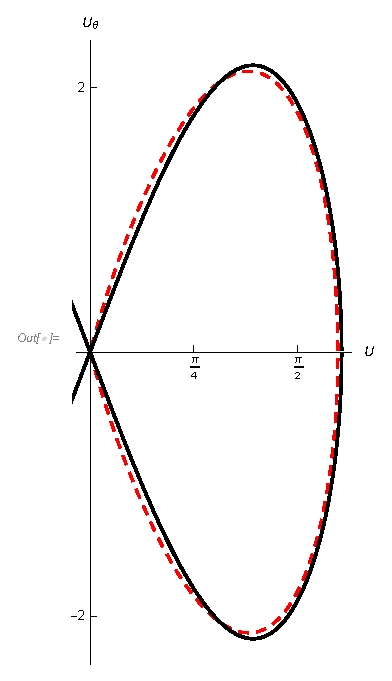
\includegraphics[width=0.75\textwidth]{images/boundary_fig1.eps}
		%\caption{Homoclinic tarjectory of the solution to Eq. (\ref{simeq4}) (solid liane) and the trajectory of target function (\ref{target}) (dashed line).}
		\caption{Гомоклиническая траектория решения уравнения (\ref{simeq4}) (сплошная линия) и траектория целевой функции (\ref{target}) (пунктирная линия).}
		\label{bound_figure1}
	\end{center}
\end{figure}
%Typical profile of the phase portrait of Eq.(\ref{simeq4}) is shown by solid line in Fig.1. However, traveling wave solutions exist under specific initial conditions. Recently the method of control of the wave localization has been developed in \cite{fradkov, porant16,  porandr17}. It was found that additional control terms in the equation can support stable propagation of nonlinear localized waves. In our case the control terms may be modeled by an external loading. Indeed,  assume that  the tangential external force in Eq. (\ref{simeq1}) is
% from the article
%Typical profile of the phase portrait of Eq. (\ref{simeq4}) is shown by solid line in Fig. 1. However, traveling wave solutions exist under specific initial conditions in the form of the wave at t = 0. Recently the method of control of the wave localization has been developed in Refs. \cite{bound_fradkov, bound_porant16,  bound_porandr17}. It was found that the additional control terms in the equation can support stable propagation of nonlinear localized waves even if the initial conditions are far from those required for the traveling wave existence without control. In our case the control terms can be modeled by an external loading on the lateral surface of the layer. Indeed, assume that the tangential external force in Eq. (\ref{simeq1}) is

Типичный профиль фазового портрета для уравнения (\ref{simeq4}) показан сплошной линией на рис. \ref{bound_figure1}. Однако решения с бегущей волной существуют при определенных начальных условиях в виде волны при t = 0. \fixme{Недавно в работах \cite{bound_fradkov, porant16, bound_porandr17} был представлен метод управления локализацией волн}. Было показано, что дополнительные управляющие члены в уравнении могут поддерживать устойчивое распространение нелинейных локализованных волн, даже если начальные условия далеки от тех, которые требуются для существования бегущей волны. В нашем случае условия управления можно смоделировать внешней нагрузкой на боковую поверхность слоя. Действительно, предположим, что касательная внешняя сила в уравнении (\ref{simeq1}) представлена в виде
\begin{equation}
	f_\tau=-\frac{k_1}{F_5}\left(q_1 F_7 U^*_x+q_2 F_{13} U^*_{xt}+q_1 F_8 u^*_x+q_2 F_{11} u^*_{xt}\right) \label{control}
\end{equation}
%where $U^*(x,t)$, $u^*(x,t)$ are the target functions. Then the r.h.s. of the first equation of motion has the form of the  control function according to the speed-gradient feedback control method \cite{fradkov, porant16,  porandr17, porant17}. Numerical sumulations reveal the stable propagation of localized waves for a particular case  Eqs. (\ref{simeq1}),  (\ref{simeq2}) \cite{porant17}. The problem is that the algorithm of control requires analytical expression for the target functions while Eqs. (\ref{simeq1}),  (\ref{simeq2}) don't have it in the general case. Then one can suggest to find the suitable expression by coinciding its homoclininv orbit with that of Eq. (\ref{simeq4}).
% from the article
%where $U^*(x,t)$, $u^*(x,t)$ are the target functions or desired waves. Then the r.h.s. of Eq. \ref{simeq1} has the form of the control function according to the speed-gradient feedback control method \cite{bound_fradkov, porant16,  bound_porandr17, porant17}. Numerical simulations reveal the stable propagation of localized waves for a particular case of Eqs. (\ref{simeq1}),  (\ref{simeq2}) at rather arbitrary initial conditions \cite{porant17}. However, the algorithm of control requires an analytical expression for the target functions. One can suggest to find the suitable expression by suiting its homoclinic orbit with that of Eq. (\ref{simeq4}).
где $U^*(x, t)$, $u^*(x, t)$ --- целевые функции или желаемые волны. Тогда правая часть уравнения \ref{simeq1} имеет вид функции управления с обратной связью согласно методу скоростного градиента \cite{bound_fradkov, porant16, bound_porandr17, porant17}. Численное моделирование показывает устойчивое распространение локализованных волн для частного случая уравнений (\ref{simeq1}), (\ref{simeq2}) при довольно произвольных начальных условиях \cite{porant17}. Однако алгоритм управления требует аналитического выражения для целевых функций. Можно найти подходящее выражение, совместив его гомоклиническую орбиту с орбитой уравнения (\ref{simeq4}). 
%In particular, the target functions in the form of a bell-shaped solitary wave can be suggested as
В частности, целевую функцию в виде уединенной волны колоколообразной формы можно предложить в виде
\begin{equation}
	u^*=\kappa_1 {\text{sech}}^4 (\kappa_2(x- c t- x_0)), \label{target}
\end{equation}
%Choosing the values of its parameters, $\kappa_i, x_0$, one can achieve the close trajectories shown  in Fig.1  by solid and dashed lines. equation (\ref{Uth}) is used to develop the target functions $U^*_x$ and $U^*_{xt}$. Obtained functions can be substituted into the control algorithm (\ref{control}) to study a tendence of an initial perturbation to a stable traveling wave defined by the target function (\ref{target}).
%Choosing the values of its parameters, $\kappa_i, x_0$, one can achieve the close trajectory shown in Fig. \ref{bound_figure1} by the solid and dashed lines. Eq. (\ref{Uth}) is used to develop the target functions $U^*_x$ and $U^*_{xt}$ using Eq. (\ref{target}). Obtained functions can be substituted into the control algorithm (\ref{control}) to study a tendency of an initial perturbation to a stable traveling wave defined by the target function (\ref{target}). This will be done elsewhere.
Перебирая значения ее параметров, $\kappa_i, x_0$, можно подобрать их таким образом, что траектории целевой функции $u^*$ и точного решения будут достаточно близки, как показано на рис. \ref{bound_figure1} штриховой и сплошной линиями соответственно. Уравнение (\ref{Uth}) используется для разработки целевых функций $U^*_x$ и $U^*_{xt} $ с использованием уравнения (\ref{target}). Полученные функции могут быть подставлены в алгоритм управления (\ref{control}) для изучения эволюции начального возмущения произвольной формы к устойчивой бегущей волне формы, определяемой целевой функцией (\ref{target}).

%\section{Weakly nonlinear case}
\section{Слабо нелинейный случай}
\fixme{Разделить на три части: преобразование уравнений, описание численной модели (?), численные результаты.}

%Consider small internal variations, $u_0 \ll 1$. In this case trigonometric nonlinearities in Eqs. (\ref{simeq1}), (\ref{simeq2}) can be expanded in power series. Only the leading order nonlinear terms are left. Also  consideration of the  long waves means that each order of derivation lowers the order of the term. The assumptions applied to  Eqs. (\ref{simeq1}), (\ref{simeq2})  give rise to the governing equations
%article
%Consider small internal variations, $u_0 \ll 1$, $U_{0,x} \ll 1$. In this case trigonometric nonlinearities in Eqs. (\ref{simeq1}), (\ref{simeq2}) can be expanded in power series. Consider only the leading order nonlinear terms without development of the formal asymptotic solution. Then Eqs. (\ref{simeq1}), (\ref{simeq2}) become
Рассмотрим \fixme{малые внутренние возмущения}, $u_0 \ll 1$, $U_{0, x} \ll 1$. В этом случае тригонометрические нелинейности в уравнениях (\ref{simeq1}), (\ref{simeq2}) могут быть разложены в степенные ряды. Оставляя при рассмотрении нелинейные члены только старшего порядка, уравнения (\ref{simeq1}), (\ref{simeq2}) преобразуются к виду
\[
\rho U_{0,tt}- F_1 U_{0,xx}- F_2 u_{0,xx}-F_{31} u_0 u_{0,x}=F_5 f_\tau+k_1 q_1 (F_7 U_{0,x}+F_8 u_{0,x})+
\]
\begin{equation}
	k_1 q_2 (F_{11} u_{0,xt}+ F_{13} U_{0,xt}) , \label{weakeq1}
\end{equation}
\begin{equation}
	(f_1+p)u_0+f_3 U_{0,xx}-s_{xx} u_0 U_{0,x}=0. \label{weakeq2}
\end{equation}
%Even the exact traveling wave solution to Eqs. (\ref{weakeq1}), (\ref{weakeq2}) is unknown. Then an approximate solution can be elaborated using the asymptotic slaving principle \cite{porpas}. According to it, Eq.(\ref{weakeq2}) can be resolved for $u_0$ using the above mentioned assumptions, and looking for a solution
Точное решение в виде бегущей волны для системы (\ref{weakeq1}), (\ref{weakeq2}) также неизвестно. Тем не менее, приближенное решение может быть получено с использованием \fixme{принципа асимптотического подчинения} \cite{bound_porpas}. Согласно этому принципу, уравнение (\ref{weakeq2}) может быть решено относительно $u_0$, используя вышеупомянутые предположения в виде
\[
u_0=u_{01}+u_{02}+u_{03}...
\]
%where
% from the article
%where $u_{03} \ll u_{02} \ll u_{03}$. Also consideration of the long waves means that each order of derivation lowers the order ofthe term, e.g. $U_{0,xx} \ll U_{0,x}$. This allows us to separate the terms in the weakly nonlinear Eq. \ref{weakeq2} by orders,
где $u_{03} \ll u_{02} \ll u_{03}$ и т.д.. Рассмотрение длинных волн также означает, \fixme{что каждая производная понижает порядок члена}, например $ U_{0, xx} \ll U_{0, x} $. Это позволяет разделить члены в слабонелинейном уравнении \ref{weakeq2} по степеням,
\[
\left((f_1+p) u_{01} + f_3 U_{0,xx}\right) + \left((f_1+p) u_{02} - s_{xx} u_{01} U_{0,x}\right) + \cdots = 0.
\]
%Then one approximately obtains
% Equating to zero the terms in big brackets separately one obtains the solutions for $u_{0i}$
Обнуляя слагаемые в больших скобках по отдельности, получаем решения для $u_{0i}$
\[
u_{01} = -\frac{f_3 U_{0, xx}}{f_1+p}, u_{02}= \frac{f_3 s_{xx} U_{0,x}U_{0,xx}}{(f_1+p)^2}.
\]
Таким образом, приближенное решение имеет вид
\begin{equation}
	u_0=-\frac{f_3 U_{0,xx}}{f_1+p}+\frac{f_3 s_{xx} U_{0,x} U_{0,xx}}{(f_1+p)^2}\label{weakeq3}.
\end{equation}
%Substitution of Eq. (\ref{weakeq3}) into Eq. (\ref{weakeq1}) results in an equation for $U_0$,
Подставляя (\ref{weakeq3}) в уравнение (\ref{weakeq1}) получаем уравнение для $U_0$,
\[
\rho U_{0,tt}- F_1 U_{0,xx}+ \frac{f_3 F_2}{f_1+p}U_{0,xxxx}+\frac{f_3 s_{xx} F_{2}}{2(f_1+p)^2} (U_{0,x}^2)_{xxx}+
-\frac{f_3^2 F_{31}}{2(f_1+p)^2} (U_{0,xx}^2)_{x}=
\]
\begin{equation}
	F_5 f_\tau+k_1 q_1 F_7 U_{0,x} + k_1 q_2 F_{11}U _{0,xt}\label{weakeq4}
\end{equation}

%The last equation doesn't have even exact traveling wave solution in the absence of an external loading, $f_\tau = 0, k_1 = 0$. Shown in Fig. \ref{bound_figure2} is the  evolution of an initial bell-shaped perturbation,
\begin{figure}
	\begin{center}
		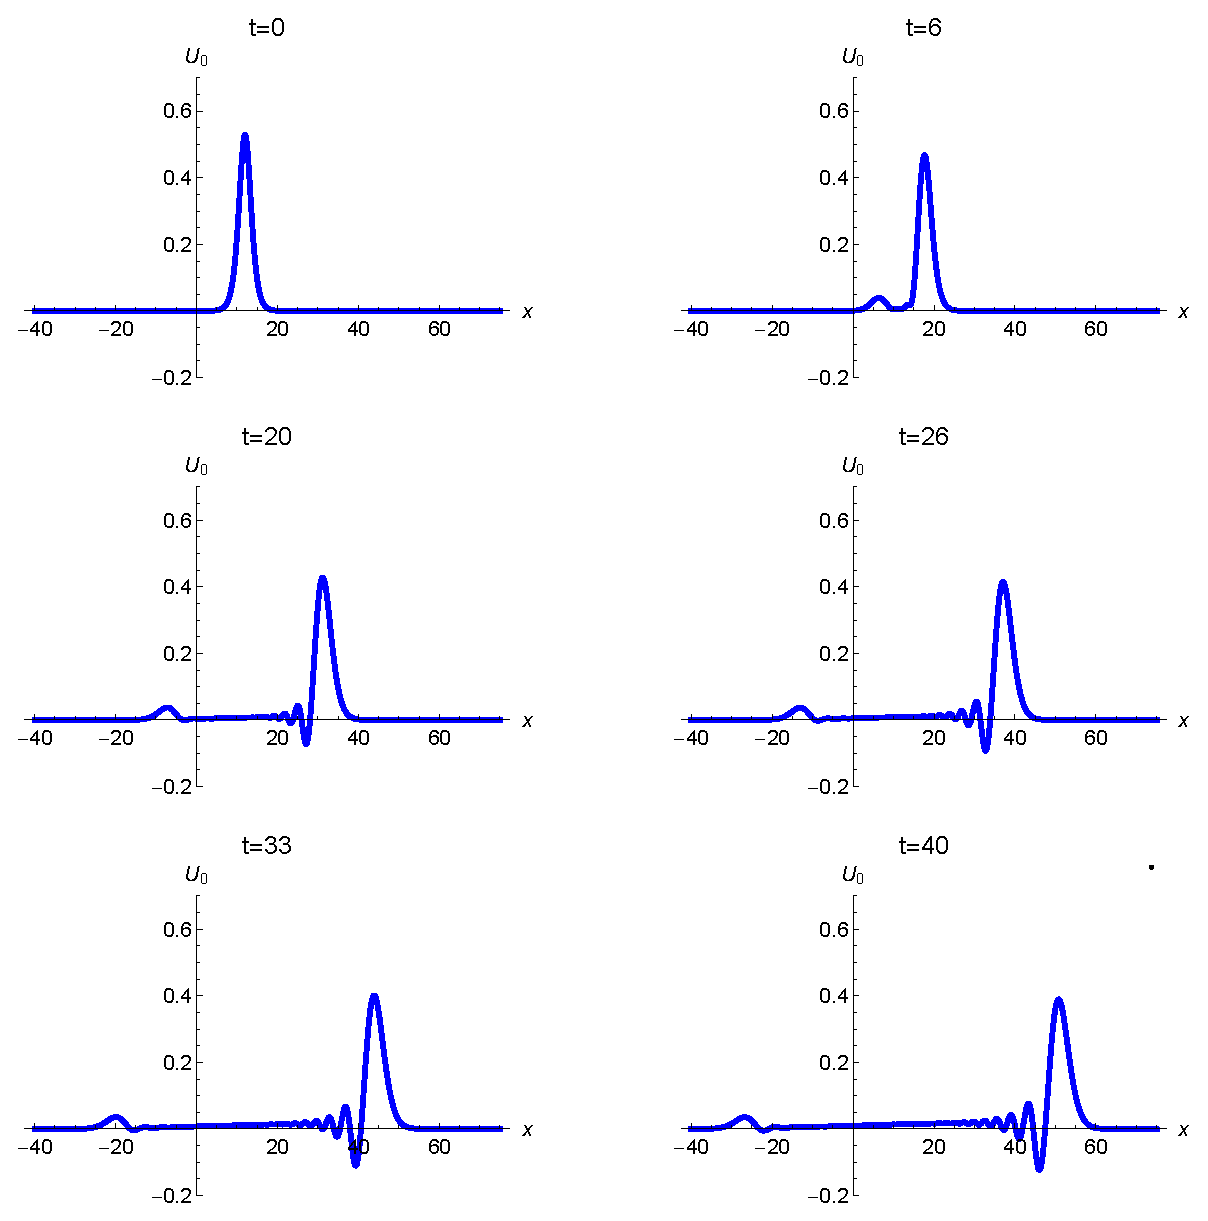
\includegraphics[width=0.95\textwidth]{images/boundary_fig2.eps}
		%\caption{Evolution of the bell-shaped input in the weakly nonlinear case  without external loading.}
		\caption{Эволюция колоколообразного начального возмущения в слабонелинейном случае без внешней нагрузки.}
		\label{bound_figure2}
	\end{center}
\end{figure} 
Последнее уравнение все еще не имеет точного решения в виде уединенной бегущей волны при отсутствии внешней нагрузки, $f_\tau = 0, k_1 = 0$. На рисунке \ref{bound_figure2} показана эволюция решения при начальном условии в виде колоколообразного возмущения следующего вида,
%\begin{equation}
$$
	U_0^*(x,0)=s_1 {\text{sech}}^2 (k (x-x_0)),
$$
$$	
	U_{0,t}^*(x,0)= s_2 {\text{sech}}^2 (k (x-x_0)) {\text{tanh}} (k (x-x_0)). %\label{target}
$$
%\end{equation}
%Here s1, s2, x0 are the constant parameters. One can see that the initial profile of U0 is not kept: the oscillations behind the wave arise, and an extra hump is developing. The former factor is caused by dispersion term U0,xxxx while the latter one appears due to nonlinear term (U20,x)xxx.
Здесь $s_1$, $s_2$, $x_0$ --- постоянные параметры. На рисунке видно, что исходный профиль $U_0$ не сохраняется в ходе эволюции: за волной возникают колебания и появляется лишний горб. Первый фактор вызван дисперсионным членом $U_{0, xxxx}$, а второй --- нелинейным членом $(U_{0, x}^2)_{xxx}$.
\begin{figure}[h]
	\begin{center}
		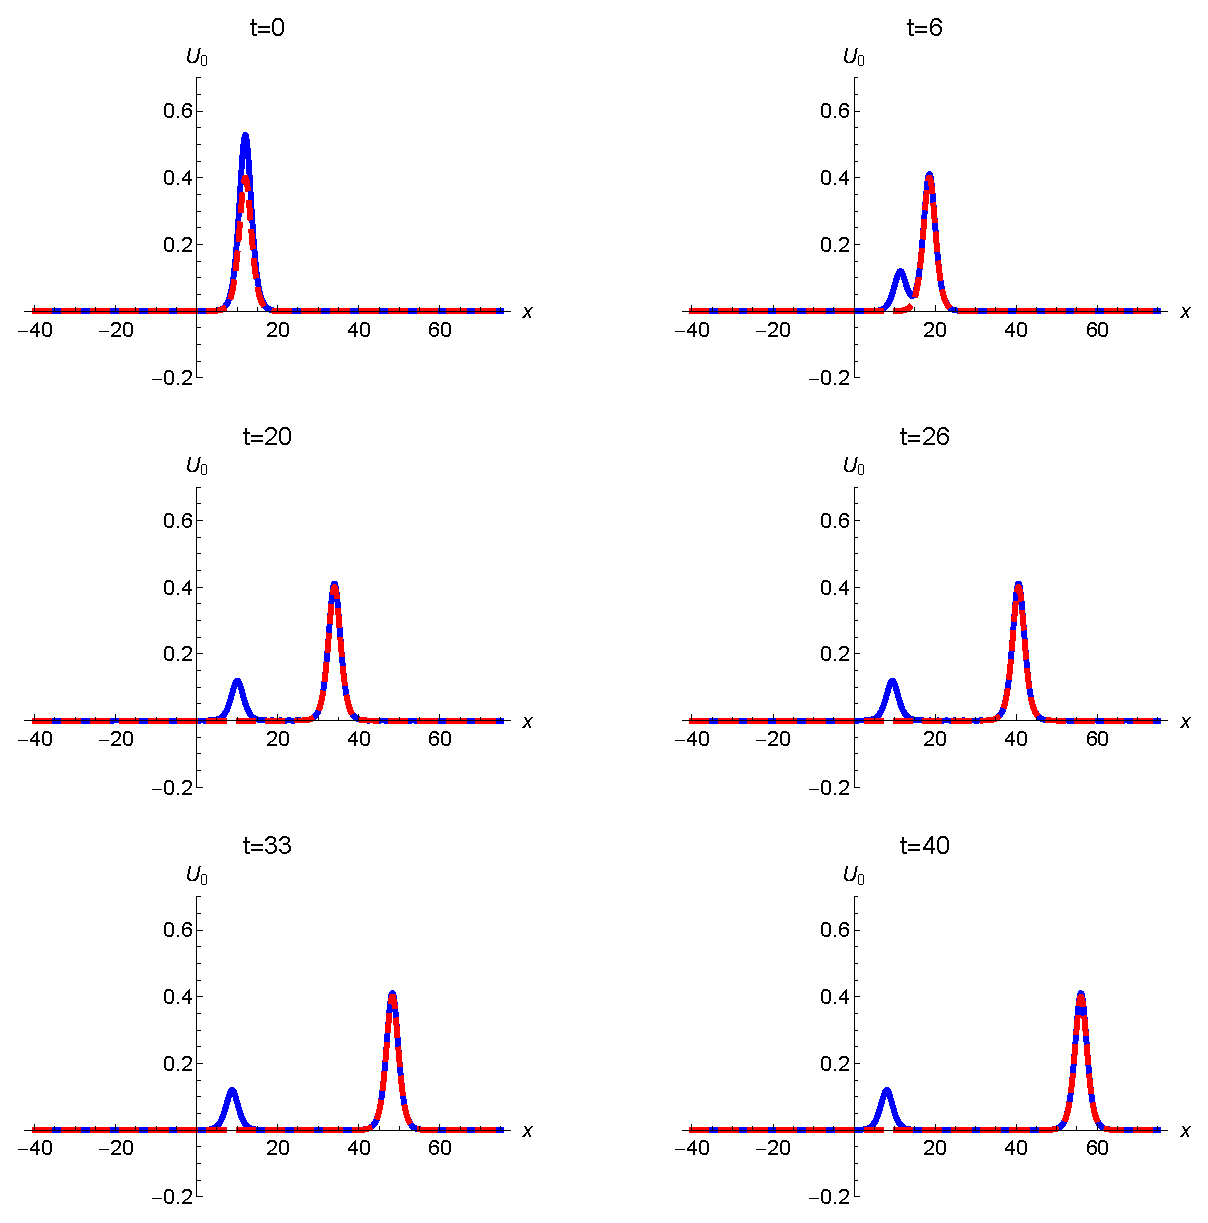
\includegraphics[width=0.95\textwidth]{images/boundary_fig3.eps}
		%\caption{Evolution of the bell-shaped input in the weakly nonlinear case  thanks to the external loading. Shown by dahsed line is the target function $U_0^*$.}
		\caption{Эволюция колоколообразного начального возмущения в слабонелинейном случае при наличии внешней нагрузки. Пунктирной линией показана целевая функция $U_0^*$.}
		\label{bound_figure3}
	\end{center}
\end{figure}
%In the absence of an external loading, $f_\tau=0$, $k_1=0$.  Here $s_1$, $s_2$, $x_0$ are the constant parameters. One can see that the  initial profile of $U_0$ is not kept: oscillations behind the wave arise, and an extra hump is developing. The former factor is caused by dispersion term $U_{0,xxxx}$ while the latter one appears due to the nonlinear term $(U_{0,x}^2)_{xxx}$. This may be checked considering particular cases with the absence of nonlinearity and the presence of only one nonlinear term.

%The presnce of an external loading changes the wave evolution as shown in Fig.3. It is assumed to consider the external force $f_\tau$ in the form
Наличие внешней управляющей нагрузки изменяет эволюцию волны, как показано на рисунке \ref{bound_figure3}. Предлагается рассматривать внешнюю силу $f_\tau$ в виде
\[
f_\tau=-\frac{k_1}{F_5}\left(q_1 F_7 U^*_{0,x}(x,t)+  q_2 F_{11} U_{0,xt}^*(x,t)\right),
\]
%where
где
\[
U^*_0(x,t)=s_1 {\text{sech}}^2 (k (x-w t-x_0)),
\]
%$w$ is a constant velocity. One can see that the r.h.s. in Eq. (\ref{weakeq4}) becomes of the form of the control function according to the speed gradient method \cite{horizont, porant16, porant17}. Temporal evolution of the function $U_0$ in Fig. 3 demonstrates fast tendency to the target function $U_0^*$ shown by dashed line. Then the stable propagation of the bell-shaped wave is observed.
%$w$ is a constant velocity. One can see that the r.h.s. in Eq. (\ref{weakeq4}) becomes of the form of the control function according to the speed gradient method \cite{horizont, porant16, porant17}. Temporal evolution of the function $U_0$ in Fig. 3 demonstrates fast tendency of the hump moving to the right to the target function $U_0^*$. We have added the target function by the dashed line in Fig. \ref{bound_figure3}, however, it is practically invisible there due to the closeness to the solid line profile of the numerical solution Then the stable propagation of the bell-shaped wave is observed.
$w$ --- постоянная скорость. Видно, что правая часть уравнения (\ref{weakeq4}) является по сути управляющей функцией согласно методу скоростного градиента \cite{bound_horizont, porant16, porant17}. Временная эволюция  $U_0$ на рис. \ref{bound_figure3} демонстрирует быструю тенденцию смещения горба вправо к целевой функции $U_0^*$. Целевая функция изображена пунктирной линией, однако она там практически не видна из-за близости к профилю численного решения. После достижения профиля волны целевой функции наблюдается устойчивое распространение колоколообразной волны, поддерживаемое управляющей нагрузкой. \fixme{Добавить описание к паразитному эффекту в виде малой медленной колоколообразной волны за профилем основной}.

\section{Заключение}
%The nonlinear strain waves may propagate in a layer made of material having a di-atomic crystalline structure. The modeling is based on the continuum approach using the expressions for the strain energy previously obtained as a continuum limit of the discrete di-atomic crystalline lattice problem. The asymptotic procedure is developed to transform an initial two-dimensional problem to a solution of  one-dimensional governing equations. In general, it is described by the coupled nonlinear equations for macro-displacements and variations in an internal structure.  The expressions for the coefficients in the equations are obtained in terms of the parameters of the original two-dimensional di-atomic lattice. The weakly nonlinear case allows us to employ a slaving principle and reduce the solution of the coupled equation to the solution of a single nonlinear equation for the macro-displacements.
%The nonlinear strain waves may propagate in a layer made of a material having a di-atomic crystalline structure. The modeling is based on the continuum approach using the expressions for the strain energy previously obtained as a continuum limit of the discrete di-atomic crystalline lattice problem. The asymptotic procedure is developed to transform the solution to the initial two-dimensional problem to the solution of the one-dimensional coupled nonlinear equations for macro-displacements and variations in an internal structure. The expressions for the coefficients in the equations are obtained in terms of the parameters of the original two-dimensional di-atomic lattice. The weakly nonlinear case allows us to employ a slaving principle and reduce the solution of the coupled equations to the solution of a single nonlinear equation for the macro-displacements.
\fixme{Исправить}

Нелинейные волны деформации могут распространяться в слое из материала, имеющего двухатомную кристаллическую структуру. Моделирование основано на континуальном подходе с использованием выражений для энергии деформации, ранее полученных в качестве континуального предела дискретной задачи двухатомной кристаллической решетки. Разработана асимптотическая процедура преобразования решения исходной двумерной задачи в решение одномерных связанных нелинейных уравнений для макроперемещений и вариаций внутренней структуры. Выражения для коэффициентов в уравнениях получены через параметры исходной двумерной двухатомной решетки. Слабо нелинейный случай позволяет использовать принцип подчинения и свести решение связанных уравнений к решению одного нелинейного уравнения для макроперемещений.

%However, the main result concerns mechanical realization of the feedback control algorithm previously formally developed in Refs. \cite{bound_horizont,bound_fradkov, porant16,  bound_porandr17, porant17}. It is shown that  an external loading acting on a lateral surface of a layer can realize the control algorithm. It allows us to support stable bell-shaped solitary wave propagation like it is seen in Fig.3. Of course, other target functions may be used instead of Eq. (\ref{target}). This was demonstrated for various nonlinear equations in our previous works \cite{porant16, bound_porandr17, porant17}.
Однако основной результат касается механической реализации алгоритма управления с обратной связью, ранее формально разработанного в \cite{bound_horizont, bound_fradkov, porant16, bound_porandr17, porant17}. Показано, что внешняя нагрузка, действующая на боковую поверхность слоя, позволяет реализовать алгоритм управления. Это позволяет поддерживать устойчивое распространение уединенной волны колоколообразной формы, как показано на рисунке \ref{bound_figure3}. Конечно, вместо уравнения можно использовать другие целевые функции (\ref{target}). Это было продемонстрировано для различных нелинейных уравнений в наших предыдущих работах \cite{porant16, bound_porandr17, porant17}.           % Глава 1
%\include{Dissertation/part1}           % Глава 1 - template
%\include{Dissertation/part2}           % Глава 2 - template
%\include{Dissertation/part3}           % Глава 3 - template
\chapter*{Заключение}                       % Заголовок
\addcontentsline{toc}{chapter}{Заключение}  % Добавляем его в оглавление

%% Согласно ГОСТ Р 7.0.11-2011:
%% 5.3.3 В заключении диссертации излагают итоги выполненного исследования, рекомендации, перспективы дальнейшей разработки темы.
%% 9.2.3 В заключении автореферата диссертации излагают итоги данного исследования, рекомендации и перспективы дальнейшей разработки темы.
%% Поэтому имеет смысл сделать эту часть общей и загрузить из одного файла в автореферат и в диссертацию:

Основные результаты работы заключаются в следующем.
%% Согласно ГОСТ Р 7.0.11-2011:
%% 5.3.3 В заключении диссертации излагают итоги выполненного исследования, рекомендации, перспективы дальнейшей разработки темы.
%% 9.2.3 В заключении автореферата диссертации излагают итоги данного исследования, рекомендации и перспективы дальнейшей разработки темы.

%\fixme{Из реферата по философии науки... Нужно исправить и дополнить.}

%В ходе проделанной работы были успешно изучены вопросы истории и методологии исследования нелинейных волновых процессов, было уделено необходимое внимание истории развития методов управления линейными и нелинейными механическими системами, при этом были подробно рассмотрены вопросы о применимости разрабатываемого математического аппарата в ходе исследовательской работы, с акцентом на методы исследования тех областей науки и техники, к которым он будет применяться в перспективе.
%Было получено полноценное представление об истории развития науки о нелинейных волнах, рассмотрены трудности, с которыми сталкивались ученые при построении новых теорий, уделено необходимое внимание появившимся в ходе этого развития новых методов исследования. В рамках данной работы также были изучены современные подходы к управлению нелинейными системами, что несомненно будет полезно для дальнейшей исследовательской работы. Таким образом, все поставленные цели работы были успешно выполнены.

\begin{enumerate}
  \item На основе анализа существующей литературы по тематике исследования были выбраны и сформулированы основные цели работы, поставлены задачи для их решения, обоснована их актуальность, практическая значимость, а также дальнейшие перспективы для развития.
  \item Разработаны модельные уравнения движения для слоя с заданными граничными условиями и видом нелинейной функции потенциальной энергии, исследована возможность управления волновыми процессами в такой механической системе по схеме скоростного градиента и определены границы применимости. 
  \item Разработан спектральный метод решения обобщенного уравнения Кадомцева-Петвиашвили с дополнительным интегральным слагаемым, описывающего распространение волн в двумерных обобщенных решетках. С помощью полученного метода численно продемонстрированы свойства устойчивости плоских волн разных типов, предсказанные аналитически. 
  \item Численно исследованы свойства распространения и генерации гармонических волн для модели метаматериала <<масса-в-массе>> в условиях наличия запрещенной зоны при различных параметрах системы. 
\end{enumerate}


%Последний параграф может включать благодарности.  
В заключение автор
выражает благодарность и большую признательность научному руководителю
Порубову~А.\,В. за поддержку, помощь, обсуждение результатов и~научное
руководство. Также автор благодарит %Сидорова~А.\,А. и~Петрова~Б.\,Б.
%за помощь в~работе с~образцами, Рабиновича~В.\,В. за предоставленные
%образцы и~обсуждение результатов, Занудятину~Г.\,Г. и 
авторов шаблона
*Russian-Phd-LaTeX-Dissertation-Template* за~помощь в оформлении
диссертации. Автор также благодарит много разных людей
и~всех, кто сделал настоящую работу автора возможной.
      % Заключение
\include{Dissertation/acronyms}        % Список сокращений и условных обозначений
\include{Dissertation/dictionary}      % Словарь терминов
\include{Dissertation/references}      % Список литературы
\include{Dissertation/lists}           % Списки таблиц и изображений (иллюстративный материал)

\setcounter{totalchapter}{\value{chapter}} % Подсчёт количества глав

%%% Настройки для приложений
\appendix
% Оформление заголовков приложений ближе к ГОСТ:
\setlength{\midchapskip}{20pt}
\renewcommand*{\afterchapternum}{\par\nobreak\vskip \midchapskip}
\renewcommand\thechapter{\Asbuk{chapter}} % Чтобы приложения русскими буквами нумеровались

\include{Dissertation/appendix}        % Приложения

\setcounter{totalappendix}{\value{chapter}} % Подсчёт количества приложений

\end{document}
